%%%% Various options for document class.
%\documentclass[usenatbib, a4paper]{preprint}
\documentclass[preprint, a4paper, 11pt]{aastex}
%%\documentclass[twocolum]{revtex4}
%%\documentclass{report}
%%\documentclass[useAMS,usenatbib, onecolumn]{mn2ejm}

%\usepackage{psfig,morefloats,url}
%use preprint2 for 2 columns paper.

%% declare any packages used
\usepackage{graphicx}
\usepackage{natbib}
\usepackage{graphicx}
\usepackage{color}
\usepackage{pdfpages}
\usepackage{appendix}
\usepackage{subfigure}
%\usepackage{epsfig}
%\usepackage[dvips]{color}
%\usepackage{aabib}


%\marginparwidth = 25pt
\citestyle{aa}
\addtolength{\topmargin}{-.5in}
%% This command added as margins are wrong in mn2e, it appears. 
%% Not needed for other classes

%% This is the end of the preamble.  Indicate the beginning of the
%% paper itself with \begin{document}.


%%%%%%%%%%%%%%%%%%%%%%%%%%%%%%%%%%%%%%

\begin{document}
%% define bibstyle and other definitions
\bibliographystyle{aabib}
%% renew commands
\renewcommand{\labelitemi}{$\bullet$}
\def\py{\textsc{Python} }
\def\tar{\textsc{Tardis} }
\def\cld{\textsc{Cloudy} }
\def\civ{C~\textsc{iv} }
\def\araa{ARAA}
\def\nat{Nature}
\def\apjl{ApJ Letters}
\def\aapr{AAPR}
\def\actaa{ACTAA} 
\def\ssr{SSR}
\def\apj{ApJ}
\def\pasp{PASP}
\def\aap{A\&A}
\def\mnras{MNRAS}
\def\aj{AJ}
\def\rmxaa{RMXAA}

%% define some control sequences for lines
\def\heiiopt{He~\textsc{ii}~$\lambda4686{\rm \AA}$}
\def\heiiuv{He~\textsc{ii}~$\lambda1640{\rm \AA}$}
\def\heiioptnew{He~\textsc{ii}~$\lambda3202{\rm \AA}$}
\def\la{Ly-$\alpha$}
\def\ha{H$\alpha$}
\def\hb{H$\beta$}
\def\civfull{C~\textsc{iv}~$\lambda1550{\rm \AA}$}

%%%%%%%%%%%%%%%%%%%%%%%%%%%%%%%%%%%%%%
%
%          TITLE AND AUTHORS
%
%%%%%%%%%%%%%%%%%%%%%%%%%%%%%%%%%%%%%%%


%\title{Modeling the Optical Spectra of Cataclysmic Variables: The Importance of Disk Winds}
\title{Disk Winds Matter: Simulating the Optical Spectra of Cataclysmic Variables}
\author{J. H. Matthews, C. Knigge, K. S. Long, S. A. Sim \& N. Higginbottom}
%%\altaffiltext{1}{School of Physics \& Astronomy, University of Southampton,
  %%Southampton, SO17 1BJ, UK}


%%%%%%%%%%%%%%%%%%%%%%%%%%%%%%%%%%%%%%
%
%          ABSTRACT
%
%%%%%%%%%%%%%%%%%%%%%%%%%%%%%%%%%%%%%%%

\begin{abstract}
High-state non-magnetic cataclysmic variables (CVs) 
exhibit strong hydrogen \& helium recombination lines in their optical 
spectra. These lines can be single peaked, and may be formed 
in the same bipolar outflow that is responsible for the
blue-shifted absorption lines seen in the ultraviolet (UV).
Here, we present results obtained by incorporating a `macro-atom' treatment into
our Monte Carlo radiative transfer code, which was
originally used to synthesize the UV spectra of disk-dominated CVs 
with a simple biconical wind. 
Using an identical model, we show that the same wind leaves a noticeable imprint 
on the optical spectrum, producing \ha\ and \heiiopt\ as well as
enhanced emission in the Ly-$\alpha$ and \heiiuv\ UV lines. 
In addition, our improved treatment of recombination means that the bound-free continuum
emission is significant, but does not yet overcome the intrinsic absorption edge
present in the stellar atmosphere models used to treat the accretion disk.
We find that a boundary layer is not essential for the production
of He II recombination lines, but also explore the effect of boundary layers
with temperatures of $80-200$kK on the ionization state of the wind
and resulting spectrum.
A short exploration of a 3-variable kinematic parameter space leads to models with higher densities 
that are able to produce single-peaked line emission, and also generate sufficient recombination emission
to fill in the Balmer jump photoabsorption edge.
Finally, we present a synthetic spectrum of a next generation model in and out of eclipse,
which shows a striking similarity with the optical spectrum of the high inclination
Nova-like variable RW Tri. The densities near the disk plane in this model
are such that \civ\ has a large collisionally excited component, in 
contrast to observations.
% We find that 
% a boundary layer is not essential to produce significant recombination to 
% He II, and if one is present we favour temperatures of $<10^5$K to avoid
% overionizing the UV resonance line species such as CIV. We also conduct Zanstra method
% calculations and estimate that one would infer a boundary layer temperature of around 80,000K
% from our benchmark calculation, despite it not being present in the model itself. This suggests that previous calculations
%done using this method are strongly dependent on both the assumed geometry and disk
%spectrum.
%We also note that
%the presence of a boundary layer becomes more noticeable in lower accretion rate systems.
\end{abstract}

\maketitle


%%%%%%%%%%%%%%%%%%%%%%%%%%%%%%%%%%%%%%
%
%          INTRODUCTION
%
%%%%%%%%%%%%%%%%%%%%%%%%%%%%%%%%%%%%%%%

\section{Introduction} 

Outflows are ubiquitous  in accreting systems across many orders of magnitude in mass,
from young stellar objects \citep{bunn1995} right up 
to quasi-stellar objects \citep[QSOs;][]{ganguly2008}. Outflows can take the form of jets, such as those
seen in X-ray binaries \citep{fender2006} or active galactic nuclei \citep[AGN;][]{marscher2006}, 
but can also manifest as `winds' emanating from the accretion disk (REFS).
Understanding the impact of accretion disk winds on spectral features has far-reaching implications. 
They provide a feedback mechanism to limit the growth of black holes in AGN \citep{silkrees1998},
and their ever-present nature implies a deep connection with the accretion process. This connection
is important to understand in order to probe the universality of accretion \citep{mchardy2006, SKUK2012} 
and to determine the true extent to which
accretion disks conform to the `$\alpha$-disk' model proposed by 
\cite{shakurasunyaev1973}. 
Despite this, in many types of systems the impact of winds on observational
features is essentially unknown, and many theoretical questions relating to their origin 
and driving mechanism remain unanswered.

Cataclysmic variables (CVs) are systems in which a white dwarf accretes matter from a donor
star via Roche-lobe overflow. In non-magnetic, disk-dominated systems this accretion
is mediated by an accretion disk which forms around the white dwarf. 
nova-like (NL) variables are a particular subclass of objects in which the accretion disk
is in a permanent state of relatively high accretion rate 
($\dot{M} \sim 10^{-8}$~M$_{\odot}$~yr$^{-1}$),
making them the perfect laboratories to test the $\alpha$-disk model.
For over three decades, it has been known that winds emanating from the accretion disk
are important in shaping the ultraviolet (UV) spectra of high-state CVs (Heap 1978), 
the most spectacular evidence being the P-Cygni like profiles of resonance lines such as 
C${\textsc {iv}}$ (see e.g. Cordova \& Mason 1982\nocite{cordova1982}).

While the effect of the wind on the UV is at least partially clear, it may also have more subtle 
effects across the spectral range. It has been proposed that an accretion disk wind
can cause single-peaked emission line profiles in the optical (Murray \& Chiang 1996), 
such as those seen in Nova-like variables and, especially, the SW Sex stars (Honeycutt, Schlegel,
\& Kaitchuck 1986; Dhillon \& Rutten 1995). It is particularly telling that single-peaked 
lines in high-inclination systems can be seen even in eclipse, suggesting 
that a spatially extensive wind may be the source of emission (see figure~\ref{novalikes}).
%%(Honeycutt, Schlegel, \& Kaitchuck 1986; Dhillon \& Rutten 1995). 
Further evidence of the influence of winds in the optical can occasionally 
be seen in P-Cygni like signatures, observed in lines such as \ha\ 
and He \textsc{i} $\lambda5876$ \citep{RN98}.
In addition, \cite{KLWB98} suggested
that recombination continuum emission from a disk wind or atmosphere
could be responsible for filling in the Balmer absorption edge. This provides
a potential explanation for
the absence of a pronounced `Balmer jump' in optical spectra of CVs, which has never been adequately produced 
by theoretical models or spectral synthesis.
This dense disk atmosphere or wind transition region
necessary to produce the required recombination emission
could also explain the Fe~\textsc{ii} `curtain'
seen in near-UV observations of the high inclination dwarf nova OY Car in quiescence 
\citep{horne1994}.


\begin{figure}	%fullpage
\centering
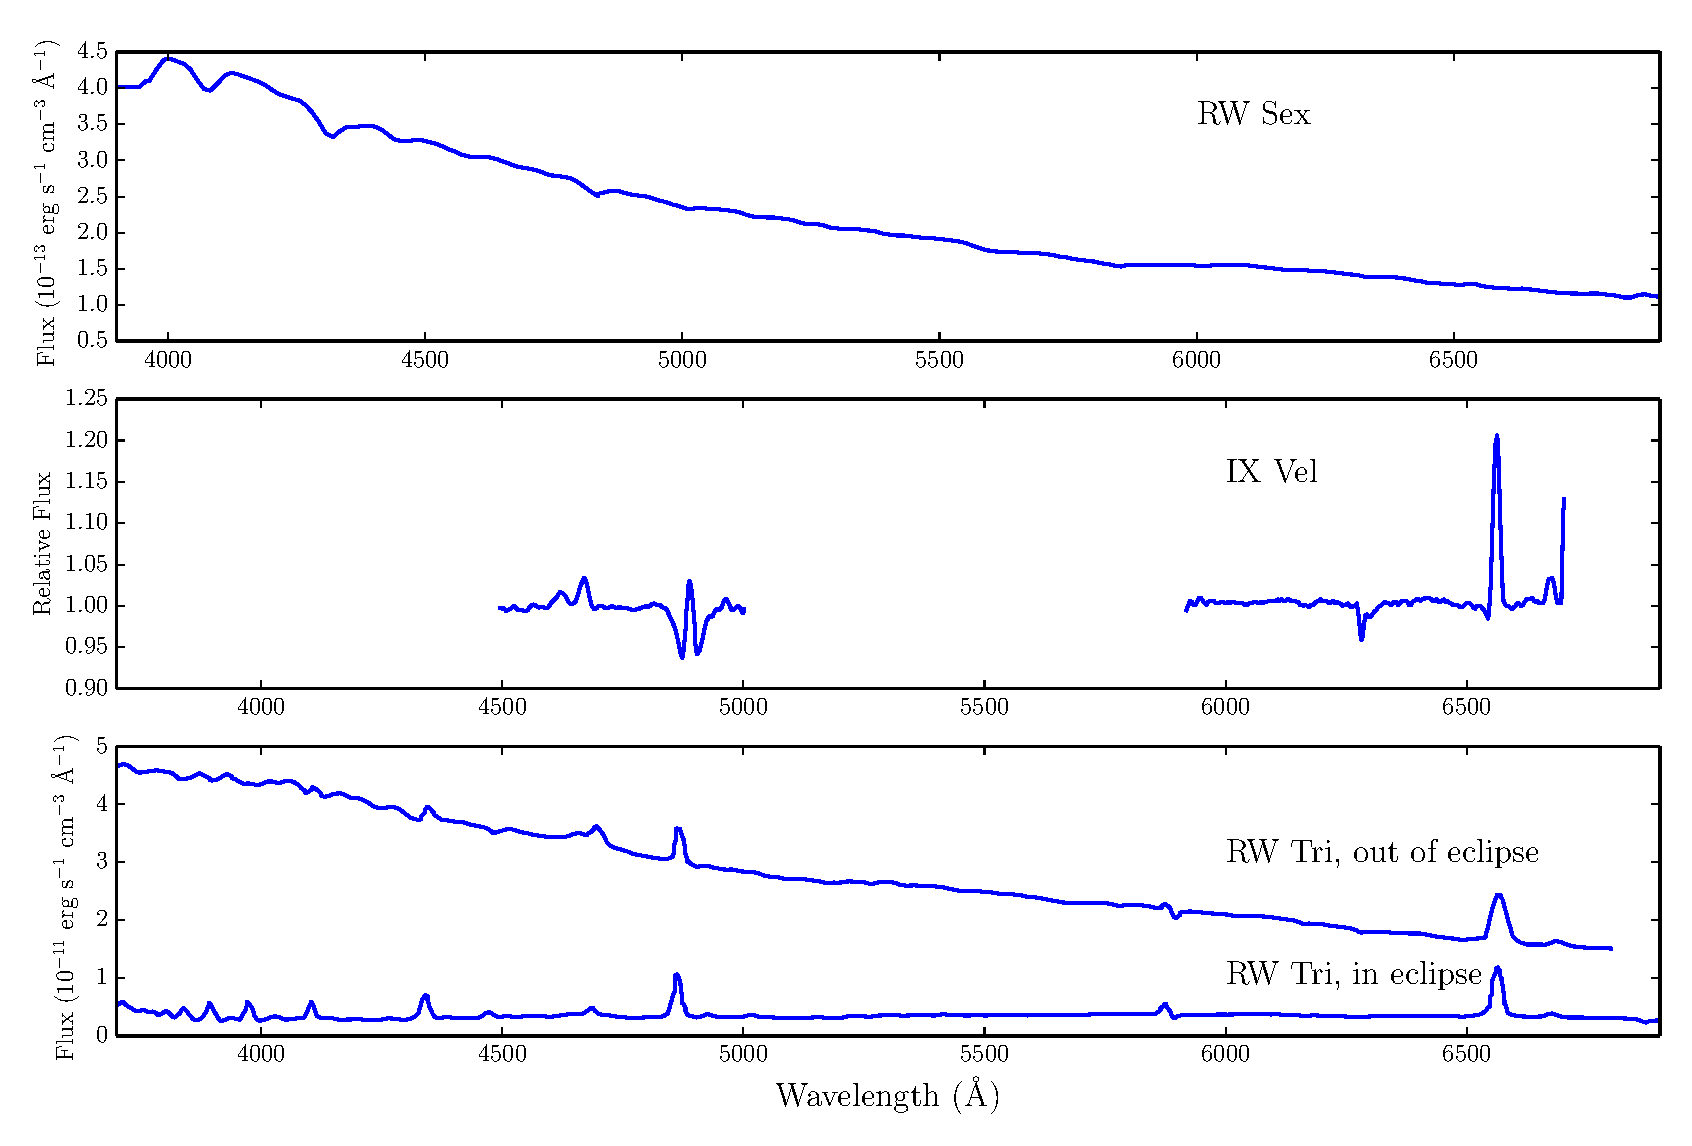
\includegraphics[width=0.8\textwidth]{figures/fig1.eps}
\caption{Optical spectra of three nova-like variables: 
RW Sex (Top; Beuermann et al. 1992),
IX Vel (Middle; Beuermann \& Thomas 1990)
and RW Tri in eclipse (Bottom; Groot et al. 2004).
The data have been digitized from the respective publications. 
These systems have inclinations of $30^\circ$, $60^\circ$ and $70^\circ$ 
respectively.
The trend of increasing Balmer line emission with inclination can be seen.
In RW Tri strong single-peaked emission in the Balmer lines is seen even
in eclipse, indicating that the lines may be formed in a spatially extensive disk wind, and there is even a suggestion
of a (potentially wind-formed) recombination continuum in the eclipsed spectrum.}
\label{novalikes}
\end{figure}

The first attempts to model disk winds in CVs applied techniques used in stellar
wind modeling to an accretion disk geometry (Mauche \& Raymond
1987; Drew 1987; Vitello \& Shlosman 1988). These efforts showed that mass loss rates of
$\sim10\%$ of the accretion rate
were required to produce the observed line strengths.
Using spectral synthesis codes to model resonance scattering,
Shlosman \& Vitello (1993; hereafter SV93) and Knigge, Woods \& Drew (1995; hereafter KWD95)
were both successful in reproducing the observed spectra such as the P-Cygni like
profiles in C\textsc{iv}~$\lambda1549$\AA.
Long \& Knigge (2002; LK02) presented a code that
solved self-consistently for thermal and ionization balance in the wind
according to the methods of Mazzali \& Lucy (1993; ML93). They successfully reproduced
UV resonance lines profiles and presented a synthesized spectrum of Z Cam
that agreed well with the observed features. Noebauer et al. (2010) used the same code 
to carry out more detailed comparisons to RW Tri and UX UMa. In addition to these 
radiative transfer calculations, some work has also been done using hydrodynamic wind models, 
such as that by \cite{pkdh2002}, and more recently by \cite{kusterer2014} with application to
AM Canum Venaticorum stars.


Here, we present work using the same Monte Carlo radiative transfer code as LK02, 
\py, but incorporating additional 
`macro-atom' techniques suggested by Lucy (2002, 2003). 
This improves our treatment of the Hydrogen and Helium
optical lines, as well as recombination continuum emission. 
Our goal is to investigate the effect of existing wind models
on the optical spectra of CVs.
In section 2 we present the code
and provide a brief description of macro-atoms and the radiative transfer methods we employ. 
We describe the kinematics and geometry of our biconical wind model in section 3.
In section 4, we present a benchmark model, which is discussed in section 5 with particular attention 
devoted to a small-scale parameter search. In section 6, we present a `next generation'
model which better reproduces the spectral features observed in NLs, and, 
finally, in section 7, we summarise our findings.

% {\bf
% \noindent Fairly happy with this as an introduction. Could maybe
% discuss the boundary layer background here instead of in section 2.
% }







%%%%%%%%%%%%%%%%%%%%%%%%%%%%%%%%%%%%%%
%
%          THE CODE, RADIATIVE TRANSFER
%
%%%%%%%%%%%%%%%%%%%%%%%%%%%%%%%%%%%%%%%

\section{Radiative Transfer}

\py is a Monte Carlo (MC) radiative transfer code which uses
the Sobolev approximation to treat line transfer. It operates 
in two distinct cycles. First, the ionization state, level populations
and temperature structure are calculated. This is done by
flying MC energy quanta (`photons') through a pre-defined wind geometry and recording
the relevant estimators, before choosing  a new electron temperature 
in an attempt to balance heating and cooling in the plasma.
This process is repeated until the code converges on a 
solution. Second, the spectrum is synthesized by tracking
the energy packets through the wind and computing the 
emergent spectra at a number of user-specified viewing angles.

The code is capable of operating in a number of different
regimes, both in terms of the scale of the system, and the 
shape and characteristic energies of the illuminating spectrum. 
It was originally described by LK02, who developed a biconical CV 
wind model to synthesize UV spectra. 
Higginbottom et al.\nocite{higginbottom2013} (2013; hereafter H13) used the same code to
present a benchmark model for broad absorption line (BAL) QSOs.
As part of this effort, the ionization scheme was improved so that 
the code is now capable of treating arbritrary SEDs.
%the power-law X-ray spectrum exhibited by AGN.
% This involved using a spectral model the mean intensity in a cell
% computed from MC estimators for, instead of using a dilute blackbody
% approximation. Compton processes
% were also incorporated into the heating and cooling balance.
In addition, \cite[][SDL05]{simmacro2005} modeled
Brackett and Pfund line profiles in YSOs using \textsc{Python,} which included
implementing a `macro-atom' mode in order to correctly treat the more
complex transition matrix involved in recombination. 



\subsection{Macro-atoms}

Previously, \py used a two-level atom approximation \cite[see e.g.][]{mihalas}. This approximation is 
fast, and works well as a first approximation when treating so-called `resonance lines' (such as C\textsc{iv}) 
in which the excited electron is strongly coupled to the ground state.
However, in a number of situations, for example, when a level is primarily populated from above, then
this becomes a poor representation. 
To reproduce recombination lines and lines in which the lower level is not the ground state, 
it is therefore important to use an improved line transfer technique and level population solver.

By quantising matter into `macro-atoms', and radiant and kinetic 
energy into indivisible energy packets (r- and k- packets respectively), 
Lucy (2002, 2003\nocite{lucy2002, lucy2003}; hereafter L02, L03) showed that it is possible 
to asymptotically reproduce the emissivity of a gas in statistical equilibrium 
without simplifying the treatment of line transfer. 
His macro-atom scheme allows all possible transition paths from a given level and a full non-Local 
Thermodynamic Equilibrium (NLTE) solution for the level populations based on MC estimators. 
For a full description consult L02 and L03. 

Macro-atoms have been used to model astrophysical plasmas in 
Wolf-Rayet star winds \citep{sim2004}, AGN disk winds \citep{simlong2008, tatum2012}
and supernovae \citep{kasen2006, kerzendorfsim}.
SDL05 used \py itself to apply this technique to
a Hydrogen-only model. We are now able to adopt a hybrid scheme. 
Any species in which have their level populations determined by
more complex interactions than resonance transitions
can be treated as full macro-atoms. The other species are treated as so-called `simple-ions',
where they still follow the indivisible packet constraint but use the two-level atom approximation.
This allows one to preserve the fast treatment of resonance lines while providing 
an improved representation of, for example, recombination, which is important when modeling features 
such as the Balmer lines and also recombination {\sl continuum} emission. 
Recombination is expected to be an important process in the optical
spectra of CVs, and they thus make a perfect application for Lucy's 
advances in MC methods.


\subsection{Ionization and Excitation}

In our hybrid ionization and excitation scheme, 
simple-ions have their ionization fractions
calculated using a modified Saha equation, and internal level populations are
calculated from LTE. For macro-atoms, we solve the equations of statistical 
equilibrium using MC estimators for the radiation field. This enables us to 
determine the ionization and excitation state of the ions in question.

\subsubsection{Macro-atoms}
% In order to correctly model lines in which the lower level is not the ground state 
% (such as H$\alpha$ \& H$\beta$), and improve the treatment of recombination,
% we treat H \& He as macro-atoms. This is because 
% the levels responsible for the line emission are populated mostly from above.
% Therefore, 
we treat H \& He as macro-atoms. 
Macro-atom NLTE level populations and ion fractions are calculated by solving 
the statistical equilbrium equations between each pair of levels. The rate
between a lower level $l$ and upper level $u$ in an ion is given by

\begin{eqnarray}
{\cal R}_{ul} &= & \beta_{lu} A_{ul} n_l + \beta_{lu} B_{ul} n_l J_{lu}^b + C_{ul} n_u n_e\label{eq:nlte_rul}\\
{\cal R}_{lu} &= & \beta_{lu} B_{lu} n_l J_{lu}^b + C_{lu} n_l n_e,
\end{eqnarray}


where $A$ and $B$ are Einstein coefficients, $C$ is the collisional rate coefficient and
$\beta_{lu}$ is the probability that a given line photon will escape the Sobolev
region. $J^b$ is the MC estimator for mean intensity at the blue wing of the line as 
recorded during the photon propagation. In the context of 
bound-free, we consider rates between the continuum state (or, in the case of ions with more than one 
bound electron, the ground state of the upper ion), $\kappa$,
and lower level $l$,

\begin{eqnarray}
{\cal R}_{\kappa l} &= & \alpha_{\kappa l} n_{\kappa} n_e \\
{\cal R}_{l \kappa} &= & n_l \int_{\nu_0}^{\infty} \frac{ 4 \pi J_{\nu} \sigma_{\nu}}{h \nu} d\nu,
\end{eqnarray}

where $\sigma_{\nu}$ is the photoioniziation cross section, $\alpha_{\kappa l}$ is the recombination
coefficient to level $l$ and $J_{\nu}$ is the mean intensity.
This treatment means that radiative and collisional rates to and from all 
levels are considered when calculating both the ionization state, and the level populations, 
although we neglect photoionization to excited levels of the upper ion. 
The \cite{vanregemorter} approximation is used for collisional transitions,
and thus we assume collisions between radiatively forbidden collisions are
negligible, a reasonable approximation in the regime where levels are mainly populated
by recombination. 
%{2002A&A...384..725L}.  source for beta sobolevs
%$\beta_{lu}=\frac{1}{\tau_{lu}}[1-\exp(-\tau_{lu})]$

\subsubsection{Two-level atoms}

C, O, N, Ne, Na, Mg, Al, Si, S, Ar, Ca \& Fe are all included as two-level atoms. 
This is a first order approximation, which is appropriate 
when treating resonance lines in which the lower level is at or close to the 
ground state. 
For these elements, we follow LK02 in using the ionization scheme presented by Mazzali \& Lucy (1993). 
Specifically, we use the formula
\begin{equation}
\frac{n_{j+1} n_e}{n_j} = W [\xi + W(1-\xi)]
\left(\frac{T_e}{T_R}\right)^{1/2}
\left(\frac{n_{j+1}n_e}{n_j}\right)^*_{T_R} \label{ionization}
\end{equation}
to solve for the relative ionization fractions. In this equation, the `starred' term on 
the right represents the Saha abundances, in accordance with the notation of Mihalas (1982). 
$W$ is an effective dilution factor, $\xi$ is the
fraction of recombinations going directly to the ground state, and
$T_R$ and $T_e$ are the radiation and electron temperature
respectively. LK02 provide a full description of our implementation.

The reason for using this scheme 
is twofold. First, unlike in H13, the SED can be approximated well by a dilute blackbody due to the 
absence of a power-law X-ray source, and therefore the above modification to the Saha equation
is appropriate; Second, this provides continuity from LK02 and allows us to do a like-for-like comparison.
This is especially useful in assessing the improvement in Hydrogen line emission, and any changes
that might occur in the ionization stages of the resonance line species such as CIV. 
Excitation is then calculated in LTE. 
%This is because the 
% level populations are only important in working out the resonance scattering 
% opacity through the wind when modeling resonance lines.



\subsection{Atomic Data}
Atomic data is obtained from the same sources described in LK02 and updated in H13. 
The additional level and line information required to treat He as a macro-atom was 
obtained from \textsc{Topbase} \citep{topbase2005}. We treat H as a 20-level atom as in SDL05, where 
each level is defined by the principal quantum number, $n$, which is appropriate due to
the degeneracy of each level in the H atom. He~\textsc{II} is treated in much the same way,
but with 10 levels. However, He~\textsc{I} has larger energy differentials between different l subshells
and triplet and singlet states. Thus, we still include levels up to $n=10$ but explicitly 
treat the $l$ and $s$ sub-orbitals as distinct levels instead of assuming they are perfectly `l-mixed',
This also allows the model to produce singlet and 
triplet lines, which are seen in optical CV spectra \citep[e.g.][]{dhillon1996}.



\subsection{Code Validation and Testing}

\py has previously been tested against a number of radiative transfer and
photoionization codes. Comparisons of ionization balance with \cld \citep{cloudy2013} 
can be found in LK02 and H13 and show excellent agreement. We have also conducted comparisons
of ionization and spectral synthesis with the supernova code \textsc{Tardis.} \tar is described by
\cite{kerzendorfsim}, and the spectral comparisons can be found therein.
In addition to these code validation efforts, we have also conducted tests of
the macro atom scheme in \py to verify that it does indeed solve for level populations correctly
and produces the expected level emissivities. Figure~\ref{tests} shows good agreement with 
l-mixed Balmer decrements in the Case B limit by \cite{seaton1959}, and 
also compares He\textsc{i} level populations with \textsc{Tardis.}

%% include figure here

% The left panel of figure~\ref{seaton} shows a comparison
% between our level emissivities for the Balmer series compared with analytic calculations
% by \cite{seaton1959}, showing good agreement in both the Case A and Case B limits 
% (see Osterbrock 1989 for a discussion of these two commonly used approximations\nocite{osterbrock}).
% The right panel of figure~\ref{seaton} shows a comparison of Helium I level populations (the most
% complex ion we currently treat as a macro-atom) between \py~and \tar~models. Considering the 
% two codes use different atomic data and \textsc{Tardis,} unlike \textsc{Python,} currently has a complete treatment of
% collisions between radiatively forbidden transitions, the factor of $<2$ agreement is 
% encouraging. 

\begin{figure}
\centering
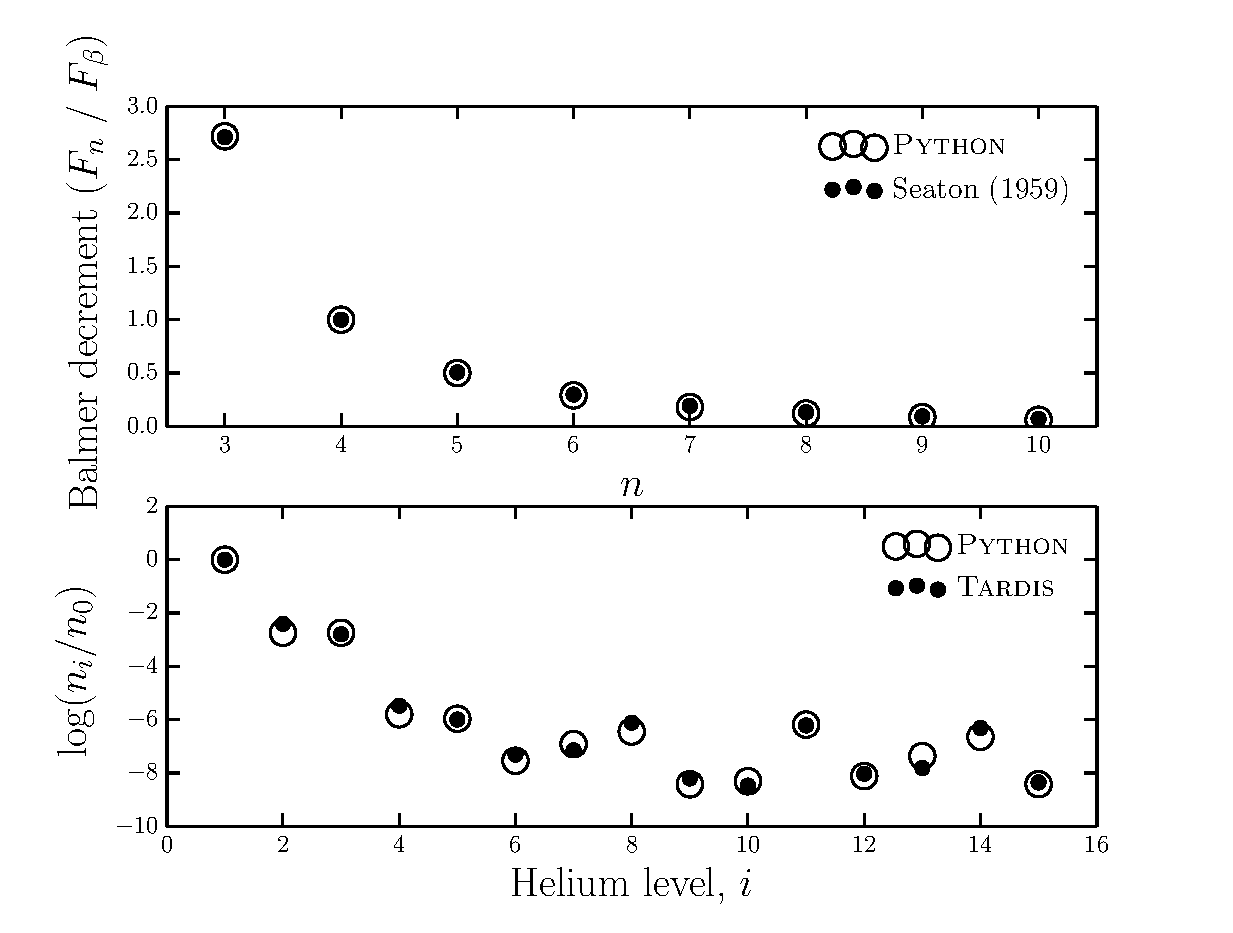
\includegraphics[width=0.5\textwidth]{figures/fig_caseb_tardis.eps}
\caption{
{\sl Top Panel:} Balmer decrements from \py compared with analytic calculations
by Seaton (1959), showing good agreement when calculating level emissivities in Hydrogen
in the Case B limit.
(see Osterbrock 1989 for a discussion of this commonly used approximation).
{\sl Bottom Panel:}  a comparison of Helium I level populations (the most complex ion we currently 
treat as a macro-atom) between \py~and \tar~models. Considering the 
two codes use different atomic data and \textsc{Tardis,} unlike \textsc{Python,} currently has 
a complete treatment of collisions between radiatively forbidden transitions, the factor of 
$<2$ agreement is encouraging. 
}
\label{tests}
\end{figure}
\nocite{osterbrock}
\nocite{seaton1959}

% \noindent\rule{16cm}{0.4pt}

% {\bf
% \noindent Notes on Section 2:

% \begin{itemize}
% 	\item Should this section go after section 3, so that we've got the reader hooked with the model description first?
% 	\item 
% 	\item Would appreciate feedback on whether explanation of macro-atoms 
% 	is sufficient.

% \noindent Potential Additional Figures:

% \begin{itemize}
% 	\item Include figure on Case A/ Case B and TARDIS comparison	
% }
%
% \noindent\rule{16cm}{0.4pt}





%%%%%%%%%%%%%%%%%%%%%%%%%%%%%%%%%%%%%%
%
%          THE MODEL
%
%%%%%%%%%%%%%%%%%%%%%%%%%%%%%%%%%%%%%%%

\section{A Biconical Wind CV Model}

Here we describe some of the features of our biconical wind model. Our aim here is not
to provide a `best fit' model to match any particular dataset.
Rather, we take as a starting point
the types of models which have already been successful in explaining UV spectra of CVs.
We can then examine the contribution of the wind to 
the optical features when the treatment of line transfer
is improved.

\subsection{Description of Model: Geometry and Kinematics}

Our model follows the prescription outlined by Schlosman \& Vitello (1993; SV93). A schematic is shown
in figure~\ref{cartoon}. A smooth, biconical
disk wind rises from the accretion disk between radii $r_{min}$ and $r_{max}$. The covering fraction of the wind is 
also controlled by the opening angles of the wind, $\theta_{min}$ and $\theta_{max}$, and the launch angle of
the other streamlines is given by

\begin{equation}
\theta(r_0) = \theta_{min} + (\theta_{max} - \theta_{min}) \left(\frac{r_0 - r_{min}}{r_{max} - r_{min}} \right)^{\gamma},
\label{theta}
\end{equation}

where $r_0$ is the launch radius of the streamline.
%As in LK02, we follow SV93's power lawvelocity profile. 
The poloidal velocity, $v_l$, in the SV93 model is given by

\begin{equation}
v_l=v_0+\left[v_{\infty}(r_0)-v_0\right]\frac{\left(l/R_v\right)^{\alpha}}{\left(l/R_v\right)^{\alpha}+1},
\label{v_law}
\end{equation}

where $l$ is distance measured along a  streamline. The terminal velocity, 
$v_{\infty}$, is set to a fixed multiple of the escape velocity at the bottom
of a streamline, and $v_0$ is a constant launch velocity (set to $6$~km~s$^{-1}$).
Once the wind is launched, it accelerates with a characteristic acceleration
length $R_v$, and $\alpha$ is an exponent which controls how quickly the 
wind accelerates. Larger values of $\alpha$ cause the main region of 
acceleration to occur close to $R_v$, whereas smaller values will lead
to a fast acceleration close to the disk (see figure~\ref{acc_law}).
SV93 chose this velocity law so as to give a 
velocity gradient that varied continuously along a streamline, as well
as producing line profiles with realistic velocity spreads.
In addition to these motivations, adopting a consistent velocity law 
allows for direct comparison with models which have already been successful in 
simulating UV resonance line profiles, such as those presented by LK02 and SV93.  


\begin{figure}
\centering
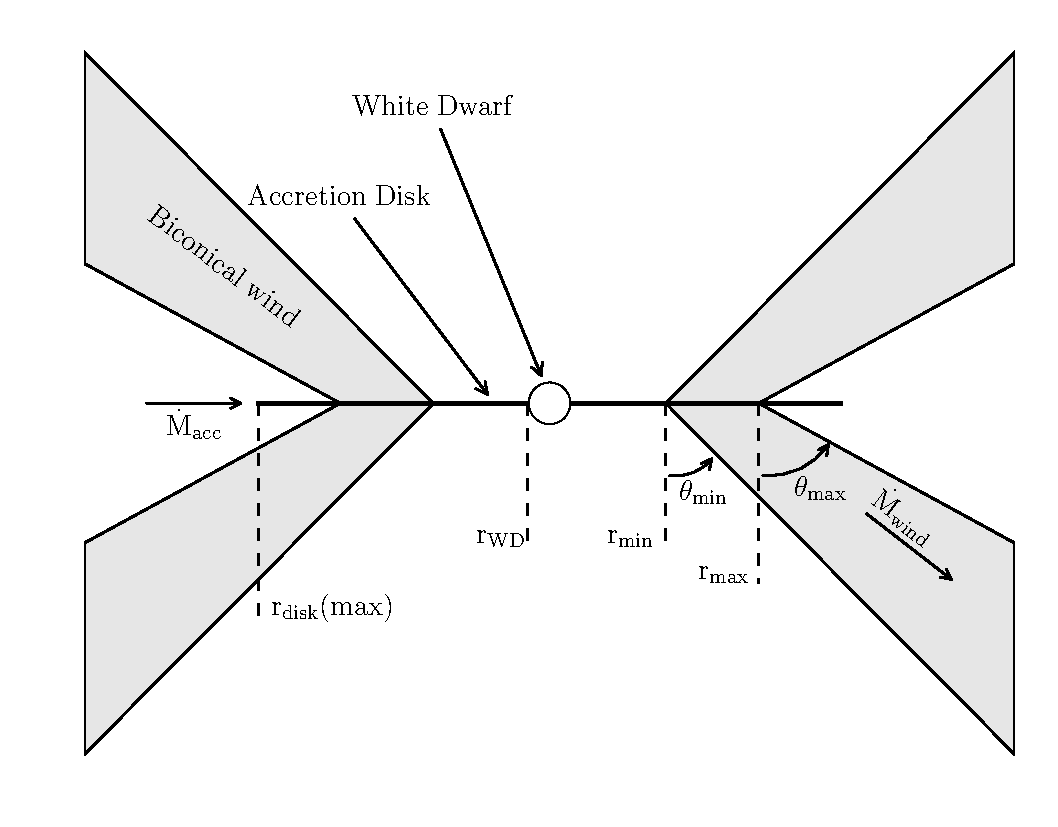
\includegraphics[width=0.5\textwidth]{figures/fig2_cartoon.eps}
\caption{Cartoon illustrating the geometry and kinematics of the benchmark CV wind model.}
\label{cartoon}
\end{figure}


\begin{figure}
\centering
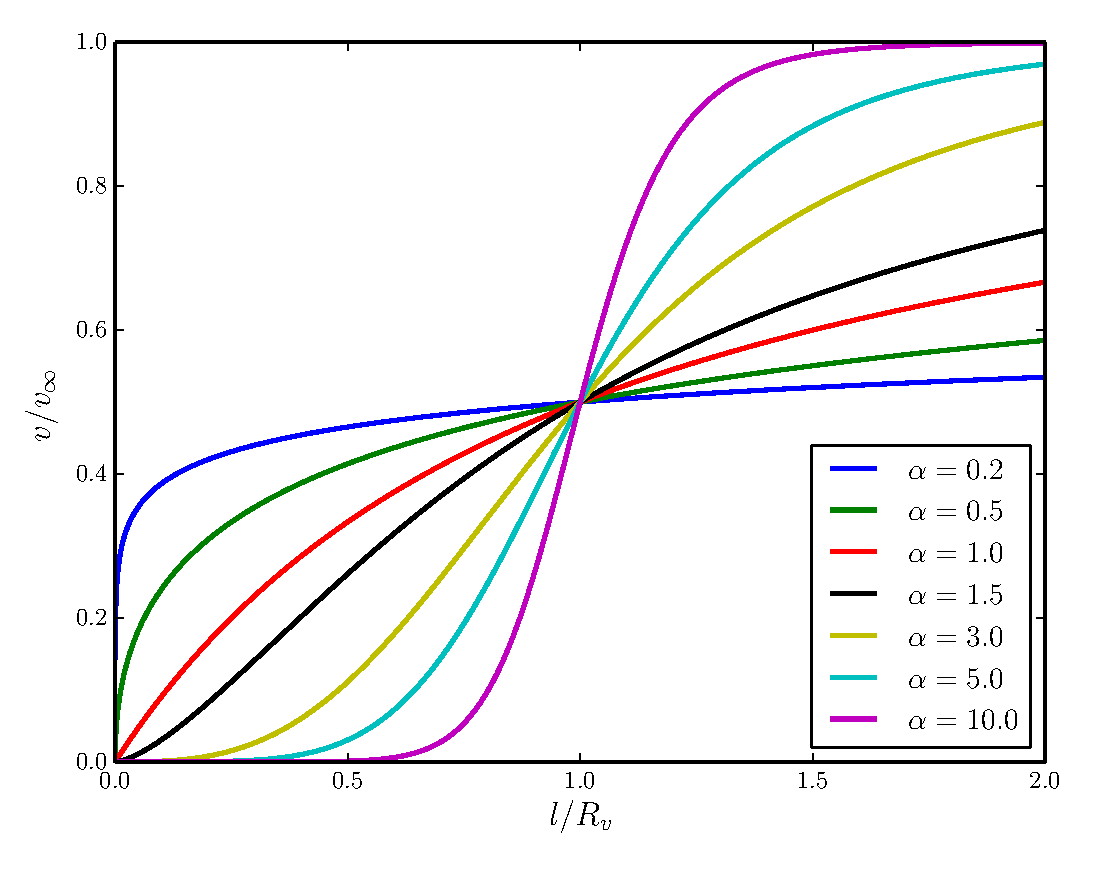
\includegraphics[width=0.45\textwidth]{figures/acc_law.eps}
\caption{
The velocity law in our model for various values of
the acceleration exponent, $\alpha$.
}
\label{acc_law}
\end{figure}


\begin{table}
\centering
\begin{tabular}{p{3cm}p{4cm}}
Model A \\
\hline Free Parameters 	&	 Value \\ 
\hline \hline 
$M_{WD}$ 	 &	 $0.8 M_{\odot}$ \\ 
$R_{WD}$ 	 &	 $7\times10^{8}$cm\\ 
$\dot{M}_{acc}$ 	 &	 $10^{-9}~M_{\odot}yr^{-1}$\\ 
$\dot{M}_{wind}$  &	fi\\ 
$r_{min}$ 	&	 $4 R_{WD}$\\ 
$r_{max}$ 	&	 $12 R_{WD}$ \\ 
$\theta_{min}$ 	&	 $20.0^{\circ}$ \\ 
$\theta_{max}$ 	&	 $65.0^{\circ}$ \\ 
$\gamma$ 	&	 $1$ \\ 
$v_{\infty}$ 	&	 $3v_{esc}$ \\ 
%%$R_v$ 	        &	 $7\times10^{10}$cm \\ 
$R_v$ 	        &	 $100 R_{WD}$ \\ 
$\alpha$ 	&	 $1.5$ \\
\end{tabular}
\centering
\caption{
Wind geometry parameters used in the benchmark CV model.}
\label{wind_param}
\end{table}


%The principle of mass conservation 
The mass continuity equation means that the velocity law also 
controls the density, $\rho$, of the wind, which can be expressed in terms
of radial and vertical position $(r,z)$ as 

\begin{equation}
\rho(r,z) = \frac{r}{r_0} \frac{dr}{dr_0} \frac{\phi(r_0)}{v_z(r,z)},
\label{density}
\end{equation}

where $\phi$ is the mass-loss rate per unit area at $r_0$
and $v_z$ is the vertical velocity component. In our model, we
adopt a uniform value for $\phi$. 



\subsection{Photon Sources}

MC quanta originate from the accretion disk and a central WD in our model. It is also possible to include
a boundary layer with user-defined temperature and emitting area. Emission from the wind is dealt with
by reprocessing of the indivisible energy packets originally produced in the disk or central WD.

\subsubsection{The Accretion Disk}

\py has has some flexibility when treating the accretion disk as a source of photons. 
The disk is broken down into annuli 
such that each annulus contributes an equal amount to the bolometric luminosity. 
We adopt the temperature profile of a standard \cite{shakurasunyaev1973} $\alpha$-disk.
%shown in figure 1.
An annulus can then
be treated either as a blackbody with the corresponding effective temperature or as a stellar atmosphere model
with the appropriate surface gravity and effective temperature. 
Both of these methods have limitations. It is known
from studies of CV accretion disks that they exhibit absorption cores 
formed in an optically thick disk atmosphere.
This can impact the overall spectrum even if a wind is present 
\citep[see e.g.][]{dhillon1996}.
However, the stellar atmosphere models
have had difficulties reproducing the required spectral shape \citep{wade1988}, 
and there are inconsistencies when using a 
stellar atmosphere beneath a dense
wind region that itself goes some way to simulating the disk atmosphere. 
In addition, \cite{linnell2010} found that deviations from the predicted 
$T\propto r^{-3/4}$ temperature profile are required to fit the data
in certain cases. 

We hope that future simulations, coupled with a comparison to data, will 
actually address some of these problems, particularly since
the filtering effect of the wind may cause noticeable effects
on the colour of the emergent spectrum \citep{hassall}. 
Here, we use a blackbody illuminating spectrum
for the ionization cycles (see figure~\ref{sed}) and to compute our MC estimators.
During the spectral synthesis stage of the simulation we use stellar atmosphere models.
This is partly because they provide the most pessimistic prediction in terms of whether recombination emission in the 
wind can fill in the Balmer jump, due to their intrinsic strong absorption beyond the Balmer edge.
For low temperatures, we use stellar atmospheres computed 
by Kurucz \citep{kurucz1991}, and for $T>50,000$~K we use models computed with 
\textsc{TLUSTY} \citep{tlusty}. The input spectra are created from these model
atmospheres using \textsc{Synspec}\footnote{http://nova.astro.umd.edu/Synspec43/synspec.html}.
%The temperature profile of our disk,
%with $\dot{M}_{acc} = 10^{-8}~M_{\odot}yr^{-1}$ can be seen in figure~\ref{t_profile}.
% more detail on why we use this hodge podge of atmosphere models?


\subsubsection{Boundary Layer}
The existence of a boundary layer in CVs arises naturally from the boundary condition
of the \cite{shakurasunyaev1973} model, since the material at the inner disk
edge must lose angular momentum in order to be deposited on
the surface of the compact object \cite[see e.g.][]{lyndenbell1974}.
Boundary layers are a possible source of
high energy photons which may be responsible for the photoionization of 
He~\textsc{ii}. 
\cite{pringlesavonije1979} predict temperatures of 
$200,000-500,000{\rm K}$ for the boundary layer,
but a number of studies have found difficulties
in producing the observed ionization state of the wind
with such a hot, luminous boundary layer 
\citep[see e.g.][]{maucheraymond1987, drewverbunt1985}.
Hoare \& Drew (1991; HD91) \nocite{hoare1991}
use the method of \cite{zanstra1929} to find upper limits on 
boundary layer temperatures of $\sim80,000{\rm K}$.


It is possible to include a boundary layer in our model which emits 
as a blackbody with the effective temperature

\begin{equation}
T_{bl} = \left[ \frac{L_{acc}}{8 \pi R_{WD} H \sigma} ( 1 - \omega_*/\omega_k)^2 \right]^{1/4},
\label{bl}
\end{equation}

where $L_{acc}$ is the accretion luminosity, $R_{WD}$ is the WD radius, $H$ is the boundary layer height
above the disk plane
and $\omega_*$ and $\omega_k$ are the angular velocities at the WD surface and inner disk edge respectively
\citep{fkrbook}. Note that we adopt a cylindrical geometry such that the effective emitting
area is $4 \pi R_* H$. 
In our benchmark model, we follow LK02 in setting the boundary layer
luminosity to zero. We investigate the effect
of boundary layers with temperatures between $80,000{\rm K}$ and $200,000{\rm K}$ 
on the ionization state of the wind and resulting
spectrum in section 5.


\begin{figure}
\centering
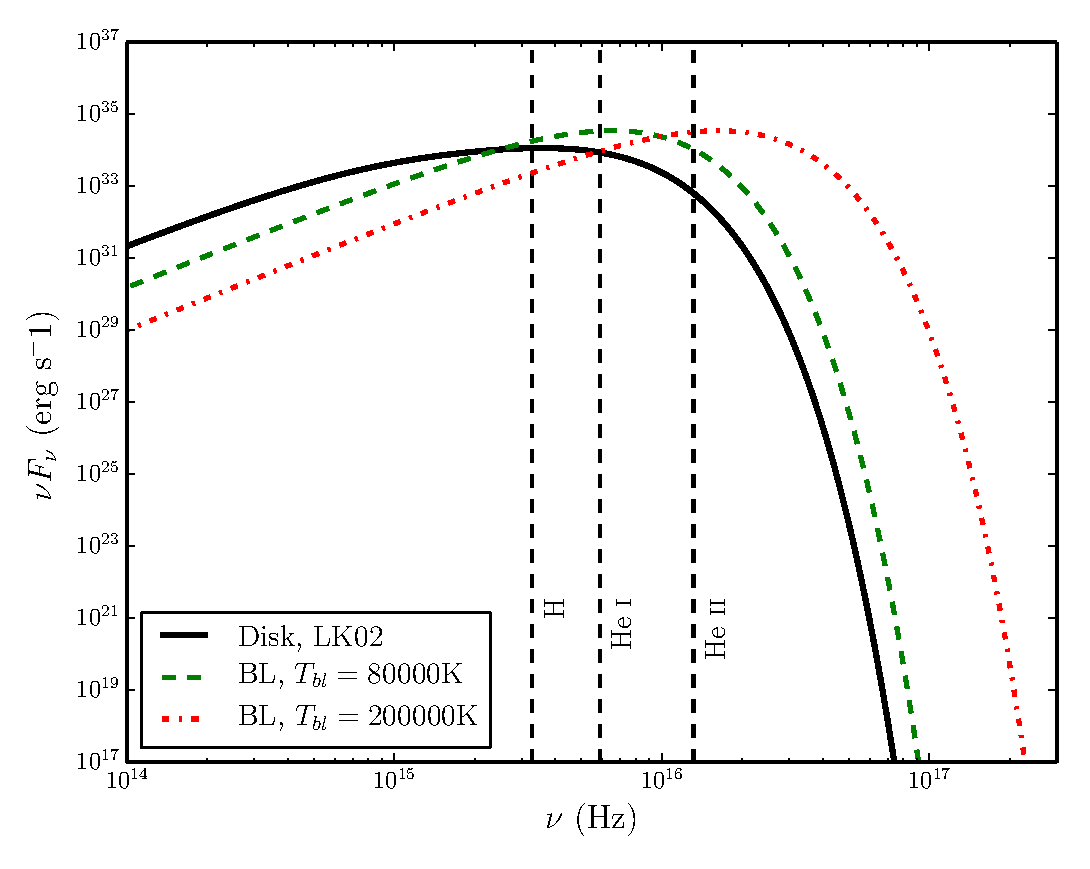
\includegraphics[width=0.45\textwidth]{figures/sed_figure.eps}
\caption{
The spectral energy distribution (SED) of the blackbody accretion
disk used in the ionization calculation (thick black line), 
with two boundary layer spectra also plotted.
The SED for an accretion disk
with the parameters used by HD91 in their Zanstra method calculations is shown in grey. 
It still assumes a Shakura-Sunyaev temperature profile, but uses
of $\dot{M}_{acc}= 5\times10^{-9}~M_{\odot}$yr$^{-1}$, and a slightly lower mass
white dwarf with $M_{WD}=0.7 M_{\odot}$ and $R_{WD} = 7\times10^{8}$cm.
The positions of the Hydrogen and Helium ionization edges 
are marked with dashed vertical lines.
{\bf NOTE: CK thinks this figure needs more discussion}.
%The effective temperature of the accretion disk
%in our model, as a function of radius.
}
\label{sed}
\end{figure}


% \noindent\rule{16cm}{0.4pt}
%
% {\bf
% \noindent Notes on Section 3:

% \begin{itemize}
% 	\item 

% \noindent Potential Additional Figures:

% \begin{itemize}
% 	\item 	
% }
%
% \noindent\rule{16cm}{0.4pt}

%%%%%%%%%%%%%%%%%%%%%%%%%%%%%%%%%%%%%%
%
%          RESULTS
%
%%%%%%%%%%%%%%%%%%%%%%%%%%%%%%%%%%%%%%%

\section{Results \& Analysis from a Benchmark Model}

The results in this section were obtained using the geometry described
in section 3. The kinematics and mass loss rate of the wind are identical
to LK02. 
% Photon sources are identical, except that when synthesizing the
% spectrum we treat the accretion disk 
% as an ensemble of Kurucz and TLUSTY stellar atmosphere models to better 
% interpret the behaviour of the Balmer jump.
The aim here is to 
take a successful UV wind model and examine its effect 
when one utilises the better treatment of lines provided
by the macro-atom scheme.

\subsection{Synthetic Spectra}

\begin{figure} %fullpage
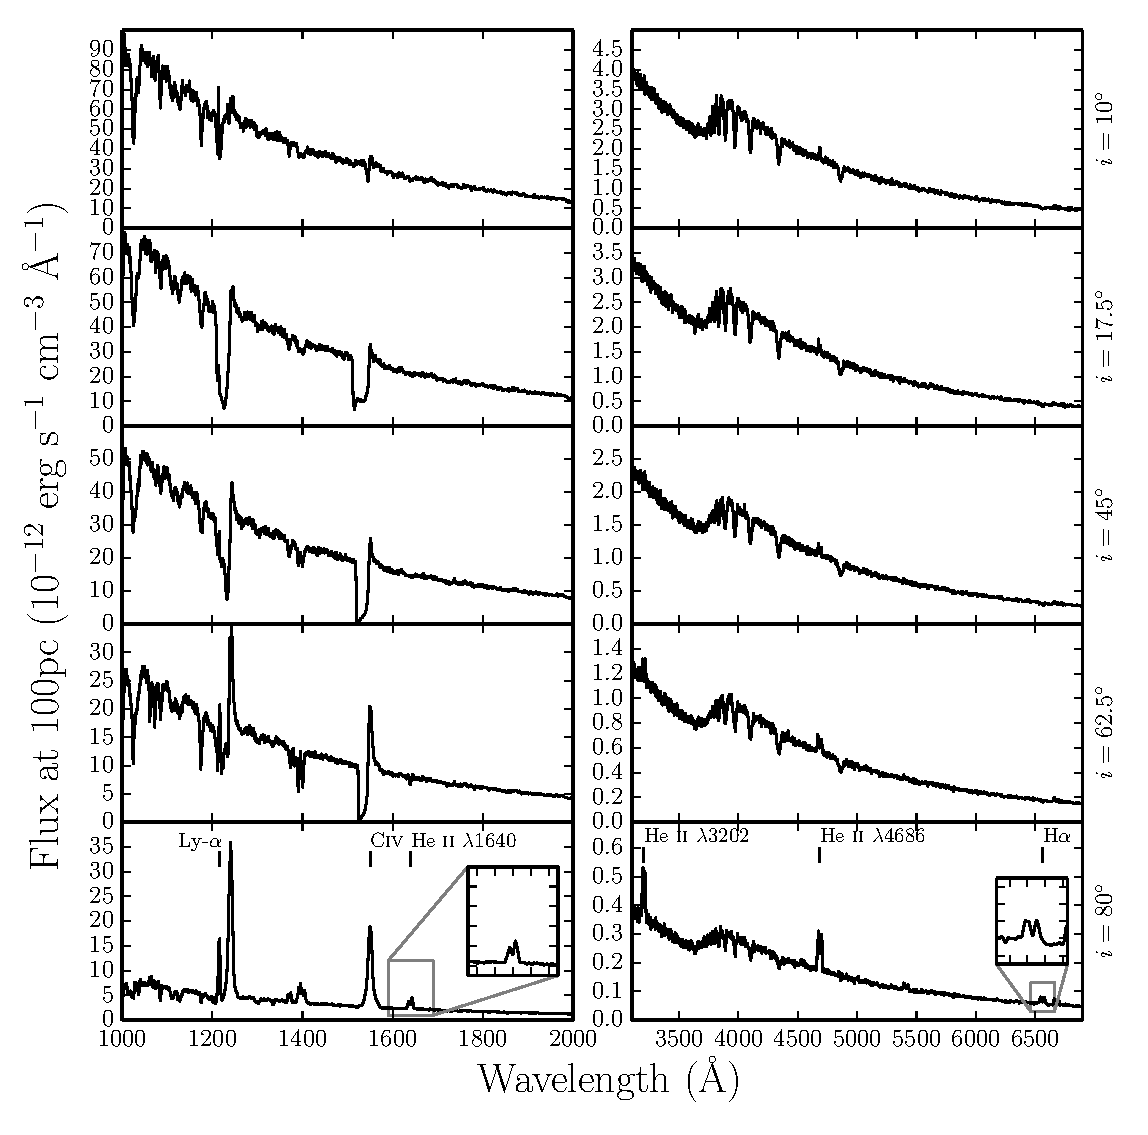
\includegraphics[width=\textwidth]{figures/fig5_uv_opt.eps}
\caption{
UV (left) and optical (right) synthetic spectra for model A, our benchmark model,
computed at sightlines of 10, 27.5, 45, 62.5 and 80 degrees.	
The inset plots show zoomed-in line profiles for 
\heiiuv and \ha. Double-peaked line emission can be seen in 
\heiiuv, \heiiopt, \ha\ and some He I lines, but the 
line emission is not always sufficient to overcome the absorption
cores from the stellar atmosphere models. The model
also produces a prominent \heiioptnew\ line at high inclinations,
}
\label{spec}
\end{figure} %fullpage\

Figure~\ref{spec} shows optical synthetic spectra for the benchmark 
model for 5 different sightlines.  
The model produces some lines which are strong enough to overcome
the absorption cores lines from the disk. These lines are generally double peaked, 
implying that they were formed near the base of the wind where rotational velocity
can still dominate over the slowly increasing poloidal velocity. 
We also see a general trend from absorption to emission in spectral lines
with increasing inclination, as one would expect from our wind geometry.
This trend is also observed in CVs and can be seen clearly in figure 1. 
Note, however,
that in our models the \heiiuv line does not exhibit this behaviour, which
is somewhat surprising. {\bf NOTE: we need to understand this!}.

The Balmer jump is in absorption at all inclinations. This is 
due to the stellar atmosphere models used to model the disk;
it is not a result of photoabsorption in the wind.
In fact, the wind spectrum has the Balmer jump in emission, 
but this is not prominent enough
to overcome the intrinsic absorption in the disk spectrum. 
Figure~\ref{cont} shows the total escaping spectrum, integrated
over all viewing angles, with the contribution from the disk and wind
shown separately. This shows that the lines are produced in the wind,
and also that the wind is producing a Balmer recombination
continuum, but one which is not yet sufficient to mask the absorption 
intrinsic to the disk SED. This offers a tantalising hint
that modest changes to the kinematics of the wind
may be sufficient to boost the continuum emission of the wind.
Furthermore, it confirms our suspicions that the improved
radiative transfer would cause enhanced recombination emission,
suggesting that, where possible, up to date treatments of
NLTE line transfer should be used in codes such as this.
The prominent P-Cygni profiles in e.g., C\textsc{iv} are still seen
in the UV spectra (see figure~\ref{spec}). In addition, the wind 
now produces significant Lyman-$\alpha$ and
He~\textsc{ii}~$\lambda1640{\rm \AA}$  emission. 
% We note that the ionization state of the wind 
% is such that recombination to He~\textsc{ii} is significant, even
% without a boundary layer as a source of higher energy photons.

In addition to examining synthetic spectra, we are also able to 
analyse the physical properties of the outflow.
Figure~\ref{wind} shows various physical properties
of the wind geometry. The ionization structure of the wind
is very similar to the original LK02 model, as one might expect.
He is mostly ionized throughout the wind except for a small region near
the disk which is shielded from the photons produced by the hot inner disk.
C\textsc{iv} is the dominant Carbon ion throughout the wind, allowing
for an absorbing column which covers a large range of velocities and is thus
sufficient to produce the required broad, deep and blue-shifted absorption lines
we expect to see in a large fraction of nova-likes.

\begin{figure} 
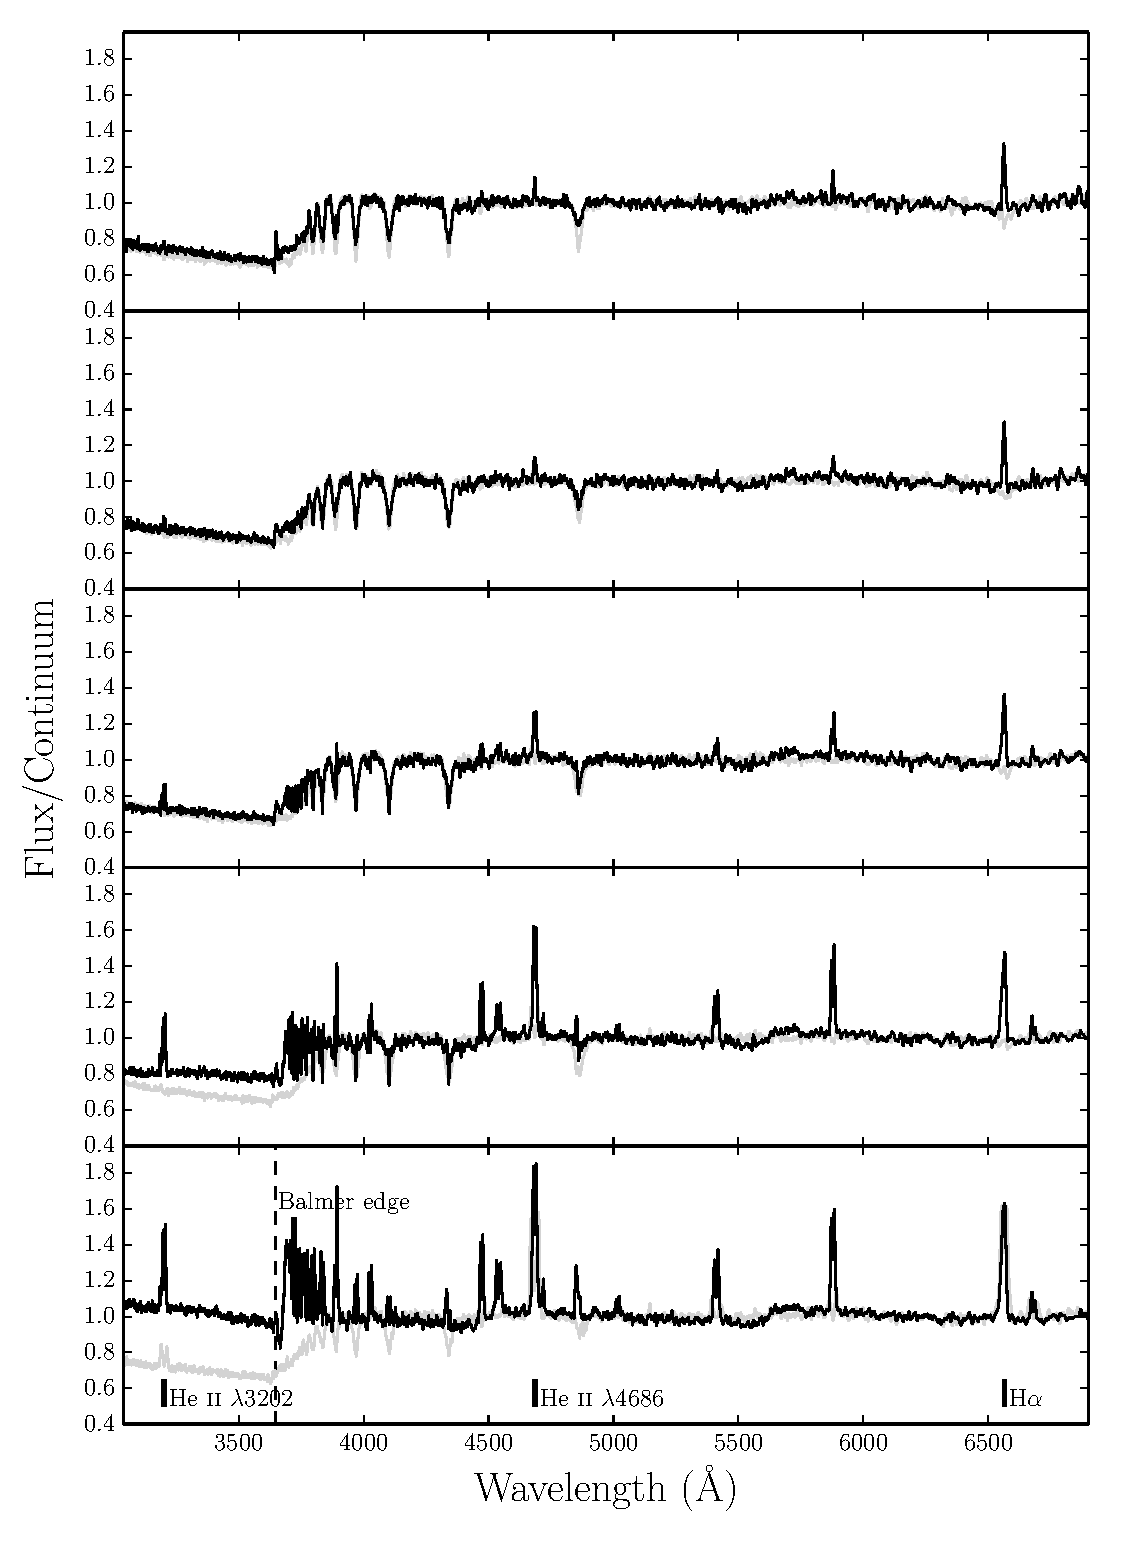
\includegraphics[width=0.45\textwidth]{figures/fig6_opt_cont.eps}
\caption{Synthetic optical spectra computed for 
sightlines of 22.5, 25, 62.5 and 80 degrees. In these plots
the flux is divided by a polynomial fit to the 
underlying continuum redward of the Balmer edge, so that 
line-to-continuum ratios and the true depth of the
Balmer jump can be shown.}
\label{spec_continuum}
\end{figure} 


Clearly, this particular model cannot explain all
the features seen in the optical spectra of nova-like variables. However,
the wind has a significant effect on the observed spectral features. 
It cannot be ignored as a source of line and continuum emission and as a reprocessing `filter'
of the underlying disk spectral energy distribution (SED).



\begin{figure} 
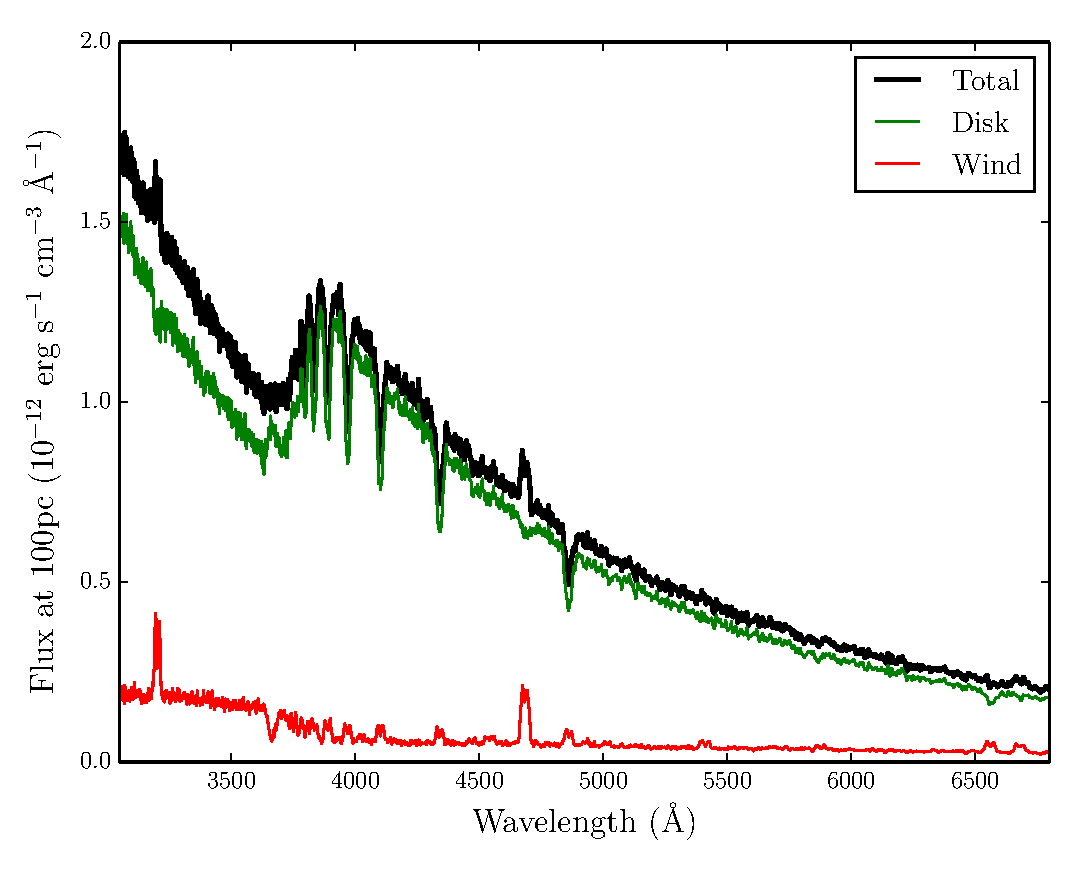
\includegraphics[width=0.5\textwidth]{figures/fig7_escaping.eps}
\caption{Total packet-binned spectra across all viewing angles. 
The thick black line shows the total 
integrated escaping spectrum, while green and red lines show the contributions from photons that originate
in the disk and wind respectively. Recombination continuum emission blueward of the Balmer 
edge is already prominent relative to other wind continuum processes, but is not sufficient
to fill in the Balmer jump in this specific model}
\label{cont}
\end{figure} 

%\subsection{Ionization and Temperature Structure}




\begin{figure} %fullpage
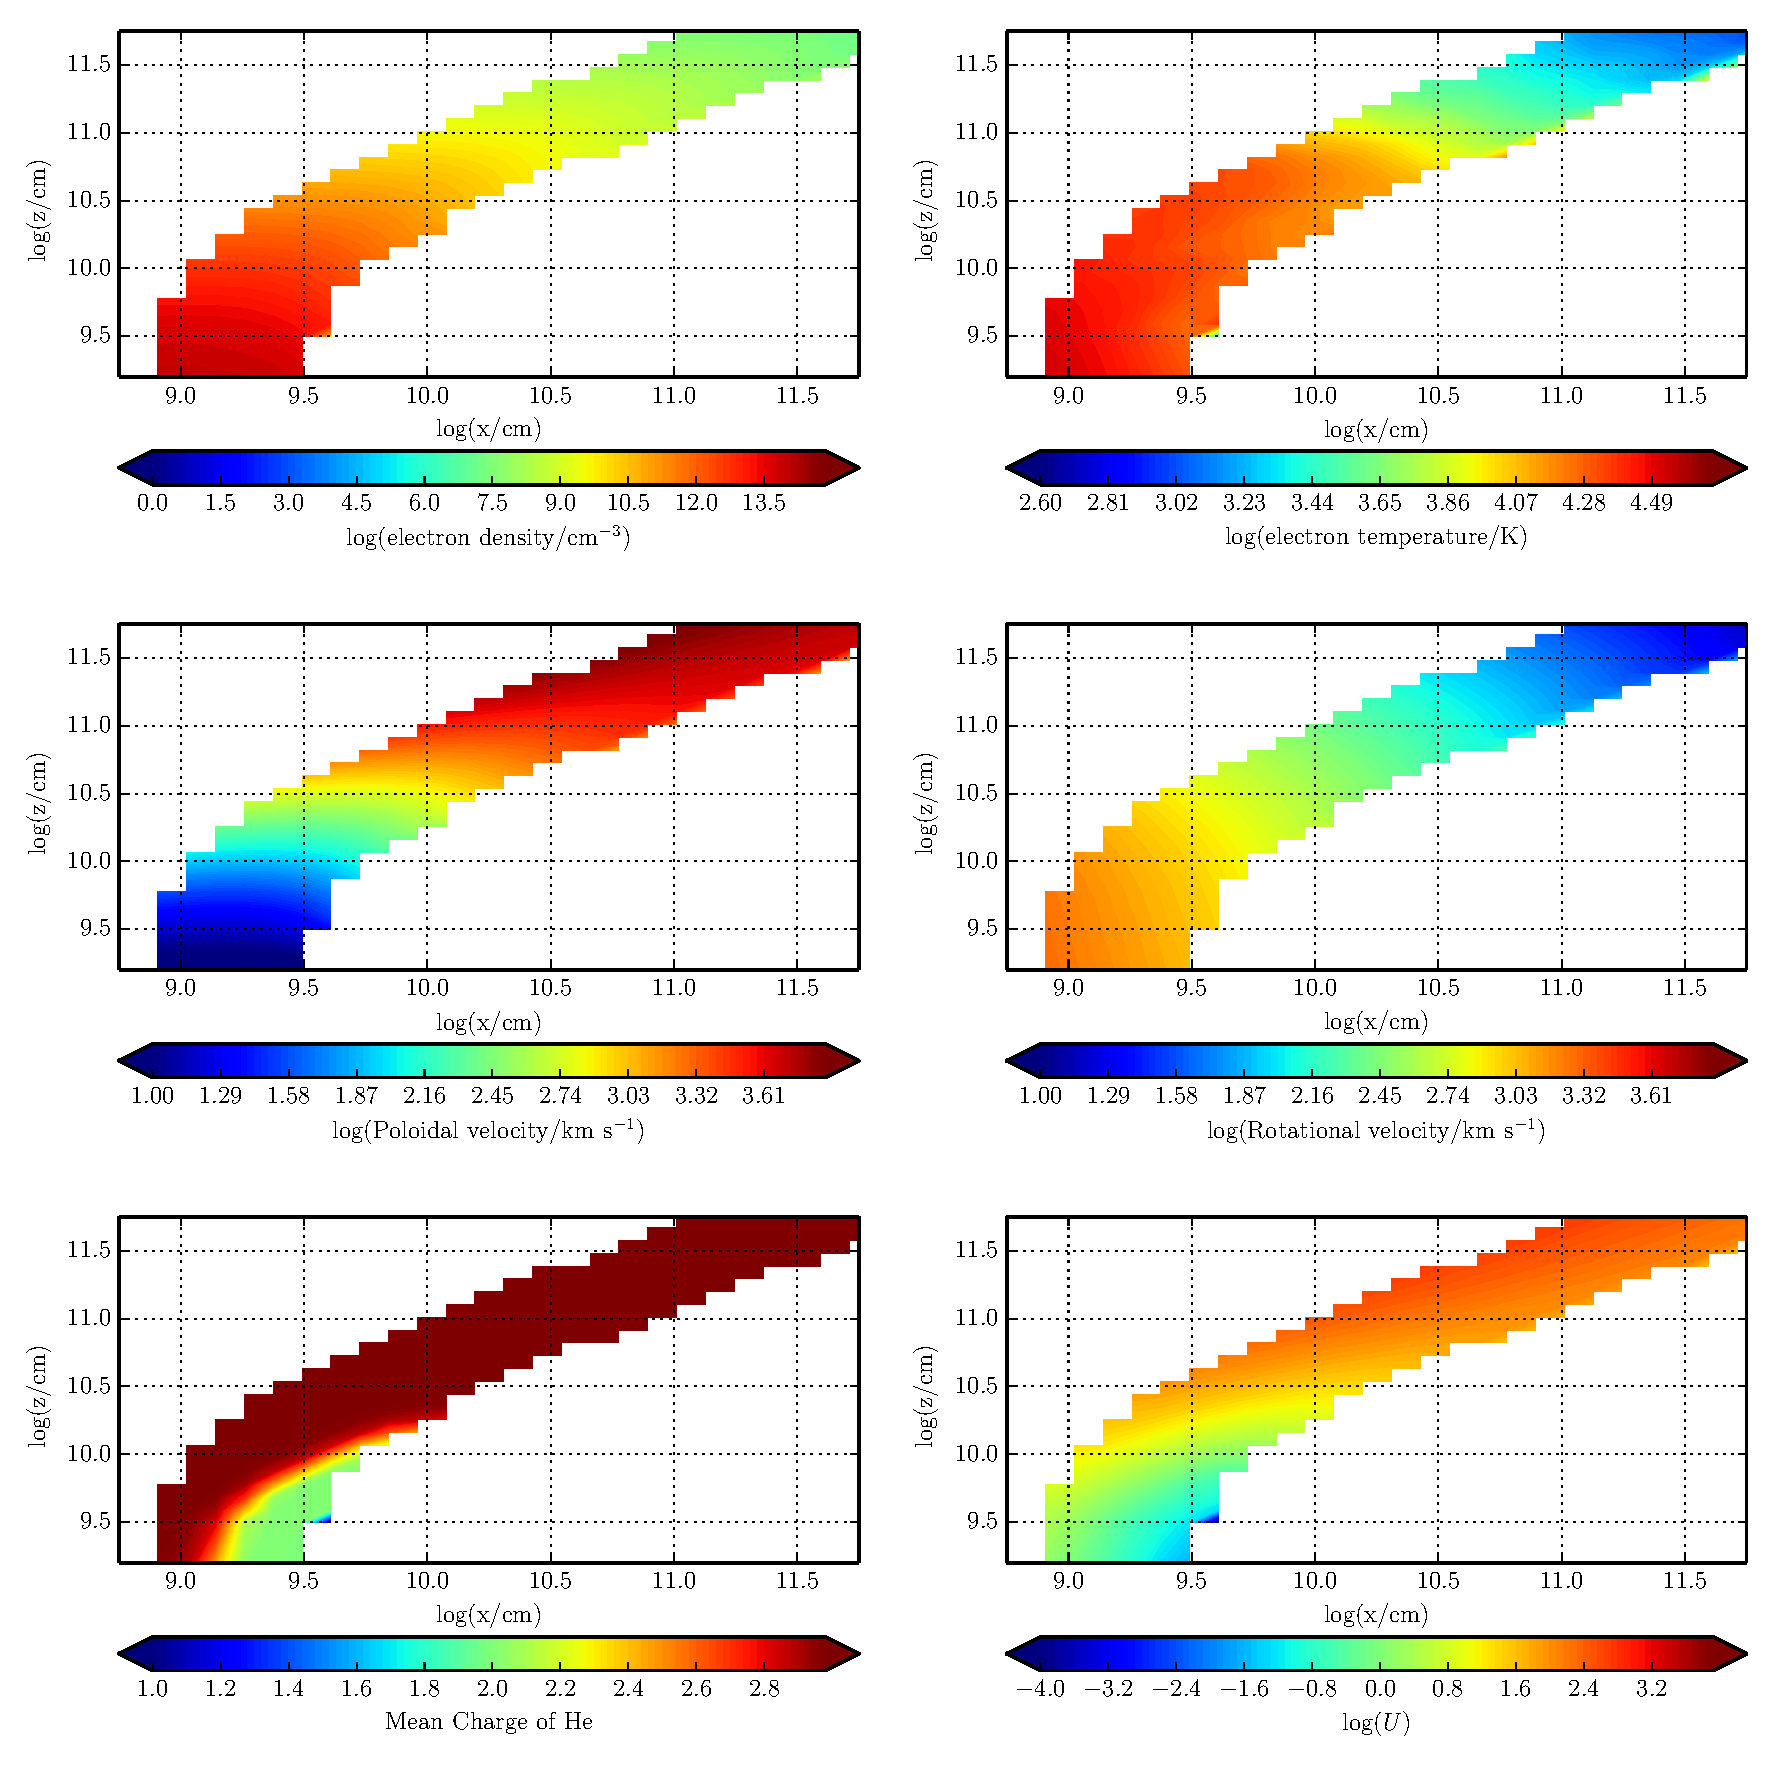
\includegraphics[width=\textwidth]{figures/fig5.eps}
\caption{
The Physical Properties of the wind. Near
the disk plane the wind is dense, with low poloidal velocities.
As the wind accelerates it becomes less dense
and more highly ionized. The dominant Helium ion
is almost always He III, apart from in a small
portion of the wind at the base, which is partially shielded
from the inner disk.
}
\label{wind}
\end{figure} %fullpage


% \noindent\rule{16cm}{0.4pt}

% {\bf
% \noindent Notes on Section 4:

% \begin{itemize}
% 	\item 

% \noindent Potential Additional Figures:

% \begin{itemize}
% 	\item 	
% }

% \noindent\rule{16cm}{0.4pt}



%%%%%%%%%%%%%%%%%%%%%%%%%%%%%%%%%%%%%%
%
%          DISCUSSION
%
%%%%%%%%%%%%%%%%%%%%%%%%%%%%%%%%%%%%%%%

\section{Discussion of Results}

The benchmark model presented above shows that a wind with the properties
of Model A, a model that successfully reproduces the observed UV spectral features
of CVs,
would also leave a clear imprint on the optical spectrum. It is important
to understand how changing the kinematics of the wind impacts on this
effect. A full parameter search is beyond the scope of this study, 
but we can examine the evolution
of the spectrum with a few key parameters. In particular, this
will help shed light on the predictions of, e.g., Murray \& Chiang (1996)
and Knigge et al. (1998) regarding the single-peaked H$\alpha$ emission
and absence of a pronounced Balmer absorption edge respectively.

\subsection{Exploring Parameter Space}

The amount of line and recombination continuum
emission produced by a given ion, $i$, in a plasma of volume $V$
depends on the emission measure, $EM$, defined as

\begin{equation}
EM=\int^V_0 n_e n_i \,dV,
\end{equation}

%% Should I quote Optical depths or 'Q' here to motivate the parameter search?

where $n_i$ is the number density of the ion in question.    
Therefore, any quantity which controls the density profile of the wind
will have a profound impact on both the 
amount of emission and the shape of the escaping line profiles.
The emission reaching an observer at a given frequency
also depends on the Sobolev optical depth it experiences, which depends on both
the density and the velocity gradient projected
along the line of sight. This can also significantly affect line profile shapes.       
As described in section 3, we can alter the density in the wind by 
adjusting the velocity law (which also determines the velocity gradient). 

We have therefore conducted a limited parameter 
sweep, exploring the effect of changing a few key parameters.  We focus on 
4 variables in order to explore the trends in our model. These are:

\begin{itemize}
 	\item the acceleration length, $R_v$, which controls the characteristic scale
 	over which the wind accelerates,
 	\item the acceleration exponent, $\alpha$, which focuses the acceleration
 	around $R_v$. A higher value of $\alpha$ therefore leads to a slowly accelerating 
 	wind with a dense base,
 	\item the launch radii of the wind, $r_{min}$ \& $r_{max}$,
 	\item the temperature of the boundary layer, $T_{bl}$.
 \end{itemize} 

We have found these to be important parameters in modifying 
the spectral features and ionization state of the wind.
In general, quantities which cause a denser wind base increase
the overal emission, although optical depth effects can cause 
the relationship to become more complicated. 



\subsection{Line Profiles: Shapes and Intensities}

% \noindent\rule{16cm}{0.4pt}

% {\bf
% \noindent key points here:

% \begin{itemize}
% 	\item producing single peaked line profiles is difficult to say the least
% 	\item with our high density models we can produce some single peaked line emission,
% 	mostly in Halpha and beta. the other lines seem to stay double peaked.
% 	\item this higher density causes (too much) collisionally excited line emission from CIV
% 	\item if the wind was more equatorial then this might help, but this isn't really supported by observations.
% 	\item we can definitely reproduce the behaviour predicted by Murray and Chiang
% 	\item Comment on the observed Balmer decrement being fairly flat, as is observed. Point out that
% 	this is necessary if H alpha is to be single peaked, as you need significant optical depths.
% 	\item \la needs to be discussed somewhere- potentially here. Personally I would like to point out
% 	that recombination being important here suggests that it might also be in QSOs
% \end{itemize}
% }

% \noindent\rule{16cm}{0.4pt}


Figure~\ref{halpha} shows how the H$\alpha$ and H$\beta$ lines change with the kinematics 
of the wind at an inclination of $80^\circ$. For H$\alpha$, in models with lower densities, the
line is double peaked, but we see a transition to a single peaked line when 
a high enough density is reach such that the line becomes optically thick.
This reproduces the behaviour predicted by \cite{MC96}, who suggested that
the poloidal velocity gradient in the wind can be larger than the gradient of 
the Keplerian velocity. This velocity gradient can therefore modify the line profile shape
by suppressing emission at the red and blue wings of the line, 
providing that the line optical depth is high enough.

In order to produce single-peaked line emission at high inclinations,
it is clear that a higher line opacity is needed at the red and blue wings relative to
the opacity at line centre. This can be achieved in a number of ways. A more equatorial 
wind would increase the radial velocity shear, but is not supported by observations (references 
on collimated nature of CV winds).
Our difficulty in producing single-peaked line emission from a full 
radiative transfer calculation has been encountered before in a number of situations. 
SDL05 found that a biconical disk geometry similar to that adopted here could not reproduce 
the observed single peaked profiles in YSOs. Here, we find
that the mechanism proposed by \cite{MC96} does indeed produce 
single-peaked line emission in our models, but for this to occur in the majority of
spectral lines very high densities are required.   

\begin{figure} %fullpage
\mbox{
\subfigure{\includegraphics[width=0.5\textwidth]{figures/grid_alpha_0.eps}}
\quad
\subfigure{\includegraphics[width=0.5\textwidth]{figures/grid_beta_0.eps}}   
}
\caption{
Line profiles for \ha\ (right) and \hb\ (left) with varying kinematic 
properties, computed for an inclination of $80^\circ$.
The benchmark model is shown in the top panel, and also in grey in each 
subsequent plot for comparison. The parameter that has been altered from the benchmark model 
is marked on each panel. For the left and middle right columns, models lower down
are more slowly accelerating and have denser wind bases. The middle right column
shows the variation with wider launch radii, and the right hand column shows 
how a boundary layer of increasing temperature affects the spectrum.
% How the H$\alpha$ and H$\beta$ lines in our model change with the kinematic properties
% of the wind. The three separate panels show three different values of $\dot{M}_W$, 
% while $\alpha$ and $R_v$ are all gradually increased from top to bottom and left to right respectively.
% Larger values of these quantities increase the density at the base of the wind. There is a clear transition
% from double peaked to single peaked behaviour, and at the highest densities the wind
% essentially becomes neutral as the optically thick regions self-shield the wind from photoionizing radiation.
% \bf{Each of these figures will highlight the next gen model in bold.
% and contain a grid like the above showing a pair of spectral features in
% the left and right panels. The grey shaded line will show the benchmark model
% for easy comparison.  
% The most promising parameters at the moment are acceleration exponent and launch radii.}
% }
}
\label{halpha}
\end{figure} %fullpage



\subsection{The Balmer Jump}

\label{balmerjump}

The left panel of figure~\ref{jump} shows the evolution
of the Balmer jump with a number of key parameters. Higher density models
produce sufficient recombination continuum emission to fill 
in the Balmer jump. This offers a potential solution to a 
longstanding problem when reconciling theoretical
models of NL spectra with observations, as originally suggested by
\cite{KLWB98}. The fact that this emission is very sensitive to the parameters
that govern the density at the wind base also supports
the idea that a transition region close to the disk plane is necessary
to explain the emission features present \citep{kd1997}.

% \noindent\rule{16cm}{0.4pt}

% {\bf
% \noindent key points here:

% \begin{itemize}
% 	\item there is always recombination continuum emission from the wind, but it
% 	only because significant w.r.t disk when the wind accelerates more slowly.
% 	\item This higher density causes (too much) collisionally excited line emission from CIV
% 	\item supports findings from the line profile shapes conclusions above...suggests
% 	we need to alter the geometry in some respect, or find someway to suppress
% 	collisionally excited line emission from UV lines?
% 	\item perhaps one should increase the volume of the emitting area rather than the density,
% 	although this will also cause more thermal line emission...
% 	\item Bottom lines: filling in the Balmer jump can be done, and at the very minimum recombination
% 	emission from the wind can matter, especially if we believe that the lines come from the wind. 
% 	But to properly fill in the edge, one requires very high, possibly unrealistic, densities.
% 	\item make clear that the edge originally comes from the stellar atmosphere, and that
% 	the model we have used here is perhaps a little pessimistic.
% 	\item We predict that the Balmer jump becomes deeper relative to the continuum 
% 	\item This is probably due to foreshortening of the disk continuum but a fairly constant
% 	escaping Balmer continuum.
% \end{itemize}
% }

% \noindent\rule{16cm}{0.4pt}


\begin{figure} %fullpage
\mbox{
\subfigure{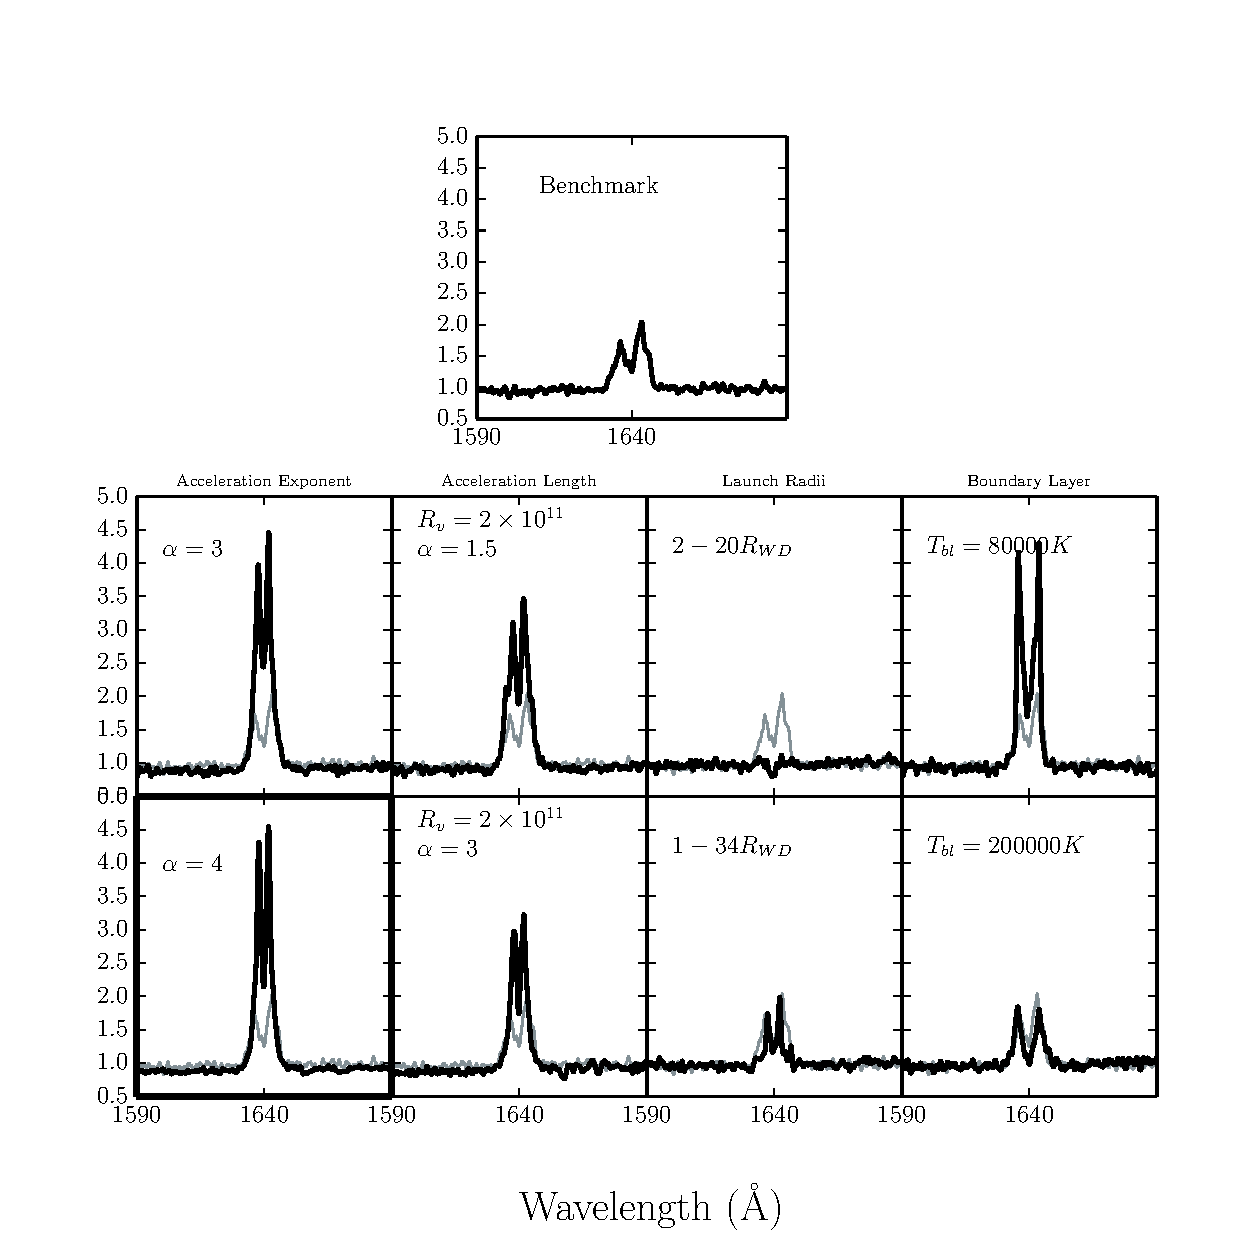
\includegraphics[width=0.5\textwidth]{figures/grid_1640_0.eps}}
\quad
\subfigure{\includegraphics[width=0.5\textwidth]{figures/grid_4686_0.eps}}   
}
%%\includegraphics[width=0.5\textwidth]{figures/test.eps}
\caption{
Line profiles for \heiiuv\ (right) and \heiiopt\  (left) with varying kinematic 
properties, computed for an inclination of $80^\circ$. 
The panels are organised in the same way as figure~\ref{halpha}.
% The panels are ordered in the same way as figure~\ref{halpha}. In general, increasing densities
% lead to a Balmer jump in emission, although as in the case of H$\alpha$ there is a transition
% when the wind becomes a neutral absorbing column.
}
\label{heiifig}
\end{figure}



\subsection{The Boundary Layer and Ionization State of the wind}

% fwoud

% important points from Hoare and Drew paper
% Zanstra method requires optically thick in He II Lyman continuum
% recombination lines are optically thin
% they note that He II n=2 edge opacity would cause more stringent limits. relevant to our edges.
% % 

% {\bf 
% \noindent key points here:

% \begin{itemize}
% 	\item we don't necessarily need a Boundary layer to ionize Helium II
% 	\item a Boundary layer of 200,000K overionizes Carbon IV
% 	\item we therefore favour lower boundary layer temperatures, as supported
% 	by the upper limits of Hoare and Drew 1991.
% 	\item we expect a boundary layer to matter more in lower accretion
% 	rate systems.
% \end{itemize}
% }

% \noindent\rule{16cm}{0.4pt}

\begin{figure} %fullpage
\mbox{
\subfigure{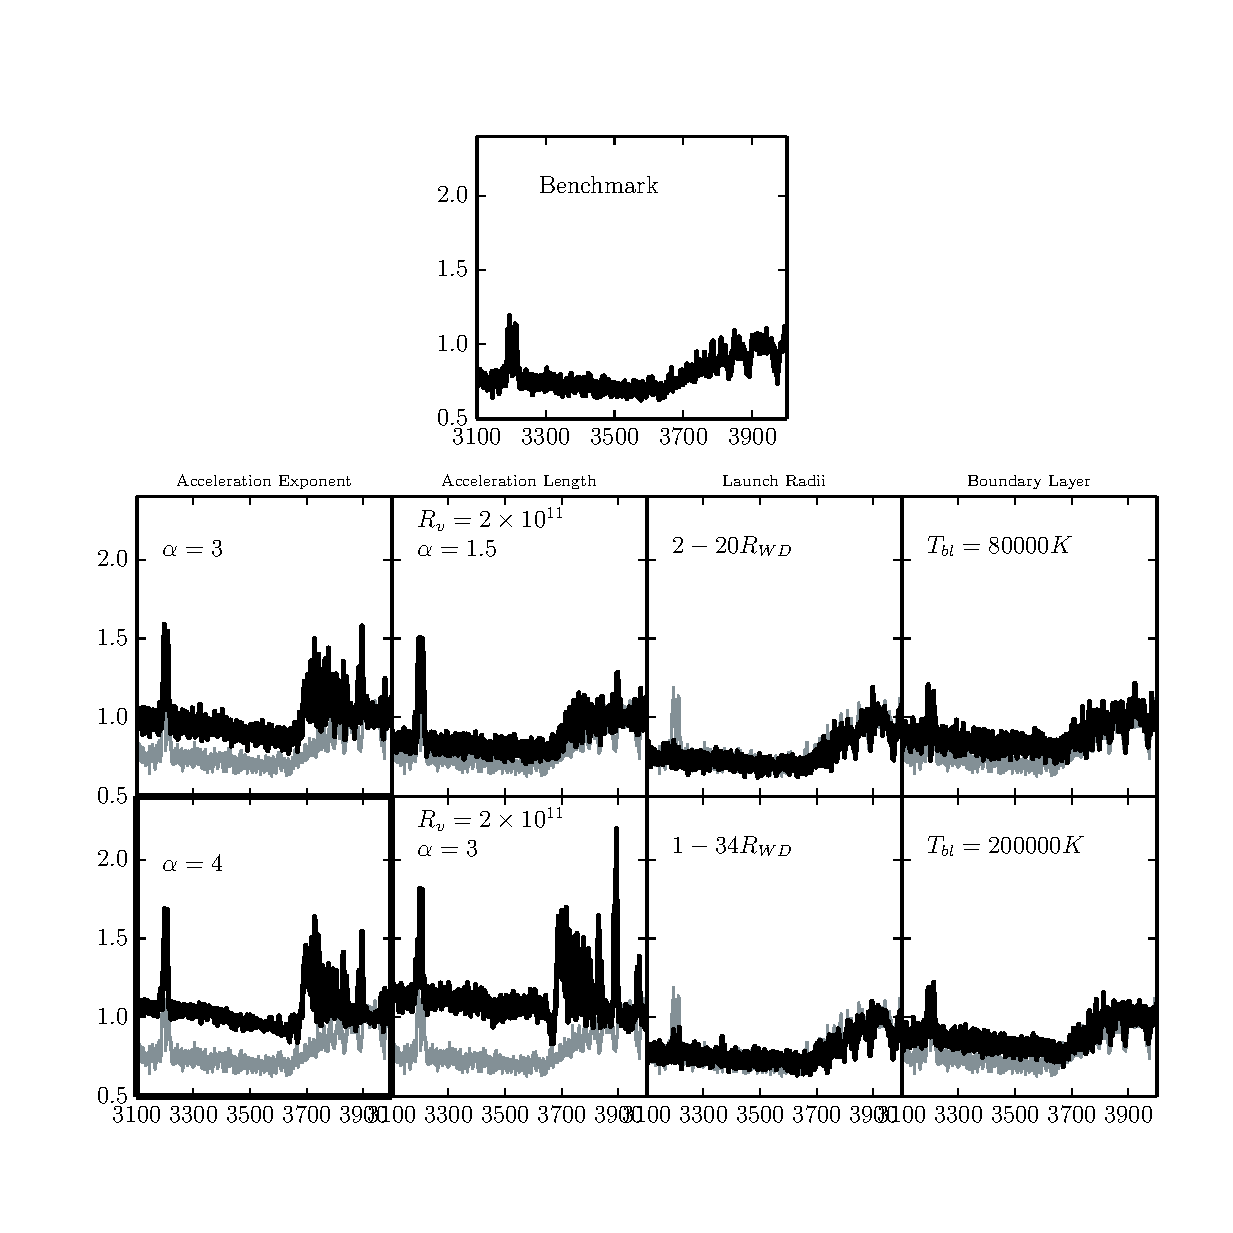
\includegraphics[width=0.5\textwidth]{figures/grid_balmer_0.eps}}
\quad
\subfigure{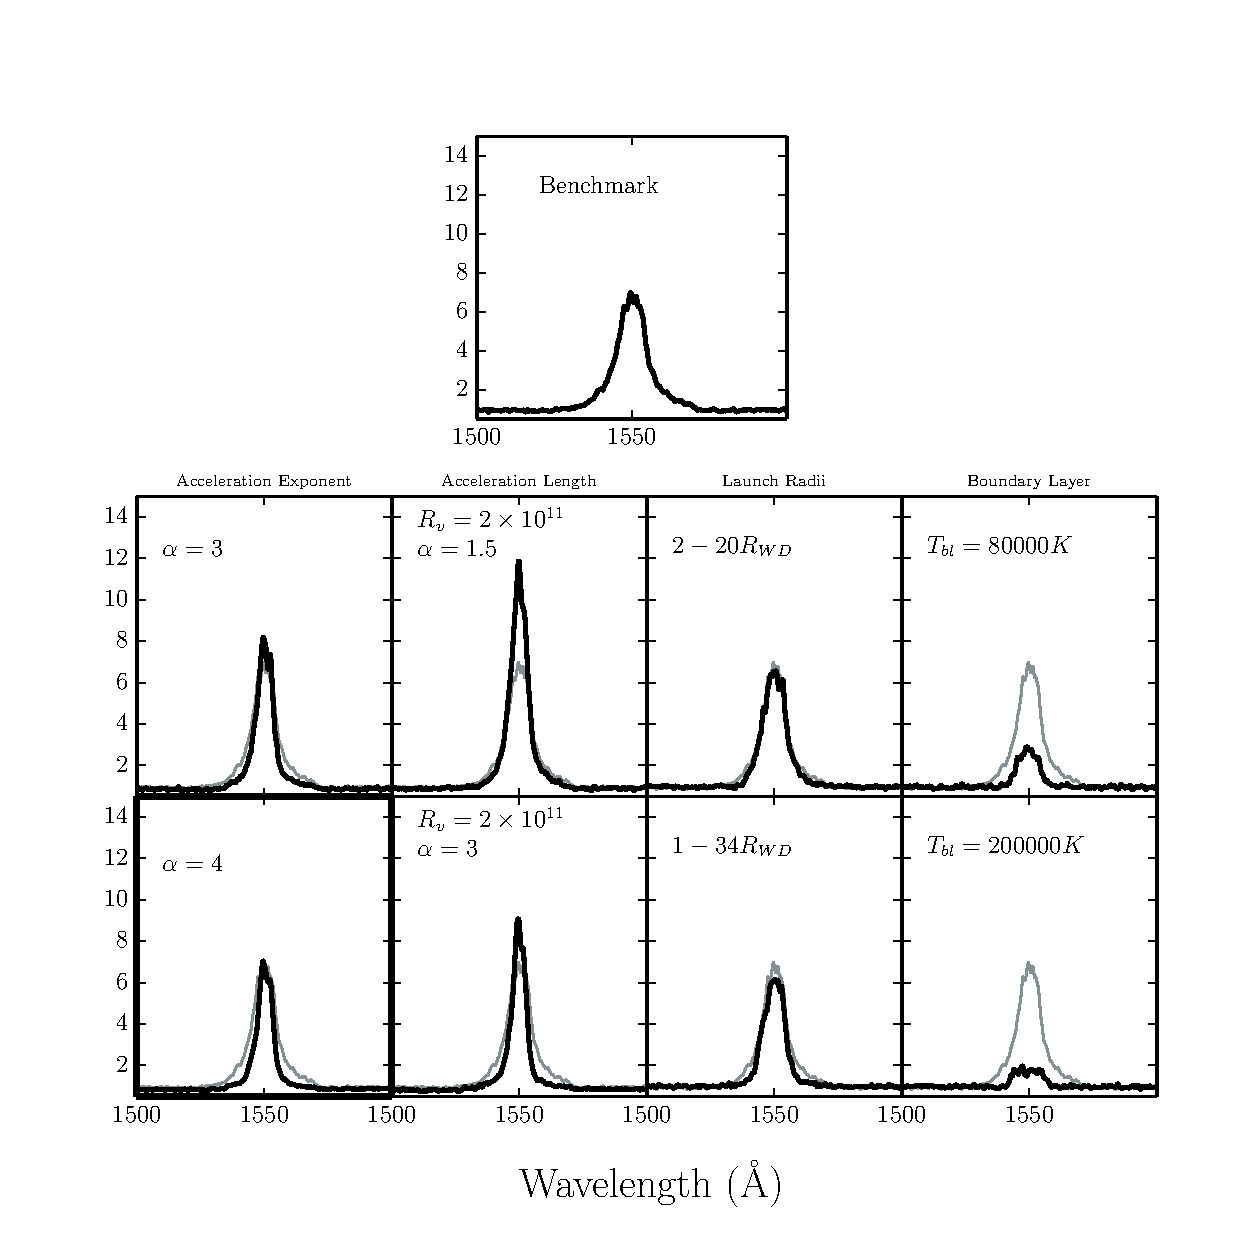
\includegraphics[width=0.5\textwidth]{figures/grid_uv_0.eps}}   
}
%%\includegraphics[width=0.5\textwidth]{figures/test.eps}
\caption{The evolution of the Balmer jump and higher order Balmer lines (left) 
and the \civ\ line profile (right)
with the kinematic properties of the wind,
computed for an inclination of $80^\circ$. 
the panels are organised in the same way as figure~\ref{halpha}.
% The panels are ordered in the same way as figure~\ref{halpha}. In general, increasing densities
% lead to a Balmer jump in emission, although as in the case of H$\alpha$ there is a transition
% when the wind becomes a neutral absorbing column.
}
\label{jump}
\end{figure}

We find in all our models that He II line emission is significant, and that 
in most cases He  III is the dominant Helium ion in the wind, making recombination
to He II an important process. This occurs without the presence of a boundary 
layer. However, as a boundary layer is theoretically predicted 
it is still important to investigate the effects of introducing
one on the ionization state of the wind, and in particular
the resultant line emission from \heiiuv, \heiiopt\ and \civ. 
We introduced blackbody boundary layers with temperatures between 80,000K and 200,000K,
commonly proposed values in the literature, and adopt a scale height according to
equation~\ref{bl}. We find that the strength of the C\textsc{iv} line decreases
with increasing boundary layer temperature. This can be seen
in figures~\ref{jump}, and also in figure~\ref{bl_grid}, which
shows the equivalent width of the \civ\ and \heiiuv\ lines as 
a function of $T_{bl}$.
We note that a model boundary layer could produce a softer
spectrum for a given effective temperature \citep[e.g.][]{suleimanov2014}, 
meaning that our ionization constraints would
allow for a higher value of $T_{bl}$.



Our findings
are consistent with calculations carried out by
\cite{hoaredrew1993}. They find that a high accretion rate 
($\dot{M}_{acc} \sim 10^{-8}~M_{\odot}yr^{-1}$) 
system does not necessarily require a boundary layer at all,
and favour cool or underluminous boundary layers
in order to explain the strengths of the \civ and N\textsc{v} 
resonance lines.
It is also possible that a flatter temperature profile in the disk,
as suggested by some eclipse mapping observations of NLs (References),
would cause a softer disk spectrum and allow a boundary layer 
with $T_{bl} = 200,000$K to exist without over-ionizing the wind.
There is an element of inconsistency with 
requiring flatter disk temperature profiles in order to permit
a hotter boundary layer, as the theoretical argument 
for the existence and likely temperature of a boundary layer has 
mostly been put together assuming a Shakura-Sunyaev disk.  
Radio emission has been seen in CVs, possibly implying the 
existence of a radio jet \cite[see e.g.][]{kordingDNjet2008,kording2011}.
A jet could extract some of the energy which is supposedly dissipated in the 
boundary layer, causing $L_{bl} < L_{acc}/2$, although
observations suggest the jet power would only be on the order
of $10\%$ of the accretion power. 
It is clear that more work is needed to understand 



% It is also instructive here to conduct a hypothetical 
% Zanstra method calculation, following the method of \cite{hoare1991}. 
% We adopt their definitions of the Zanstra ratios in the Helium lines (equations 5 and 6 
% in their paper),


% \begin{equation}
% G (\lambda228, 1800 \AA) = 2.4\times 10^{-3} \frac{f(\lambda1640)}{f_*(1800\AA)}
% \end{equation}
% and

% \begin{equation}
% G (\lambda228, 1800 \AA) = 1.3\times 10^{-3} \frac{f(\lambda4686)}{f_*(1800\AA)}.\\
% \end{equation}

% Here f(line) is the line flux in erg~cm$^{-2}$ s$^{-1}$. (I NEED TO DO THE CALCULATION!).

% Possible figure: CIV line equivalent width or ionization fraction
% as a function of boundary layer temperature?


% Discussion of Helium lines in the spectrum.
% \begin{itemize}
% \item He II 4686, He II 1640 strengths
% \item Make the prediction that if 4686 is strong we might expect strong He II 3202. 
% \item Discuss why it wouldn't have been seen yet (spectral coverage)
% \item Helium I lines
% \end{itemize}




\begin{figure} 
\mbox{
\subfigure{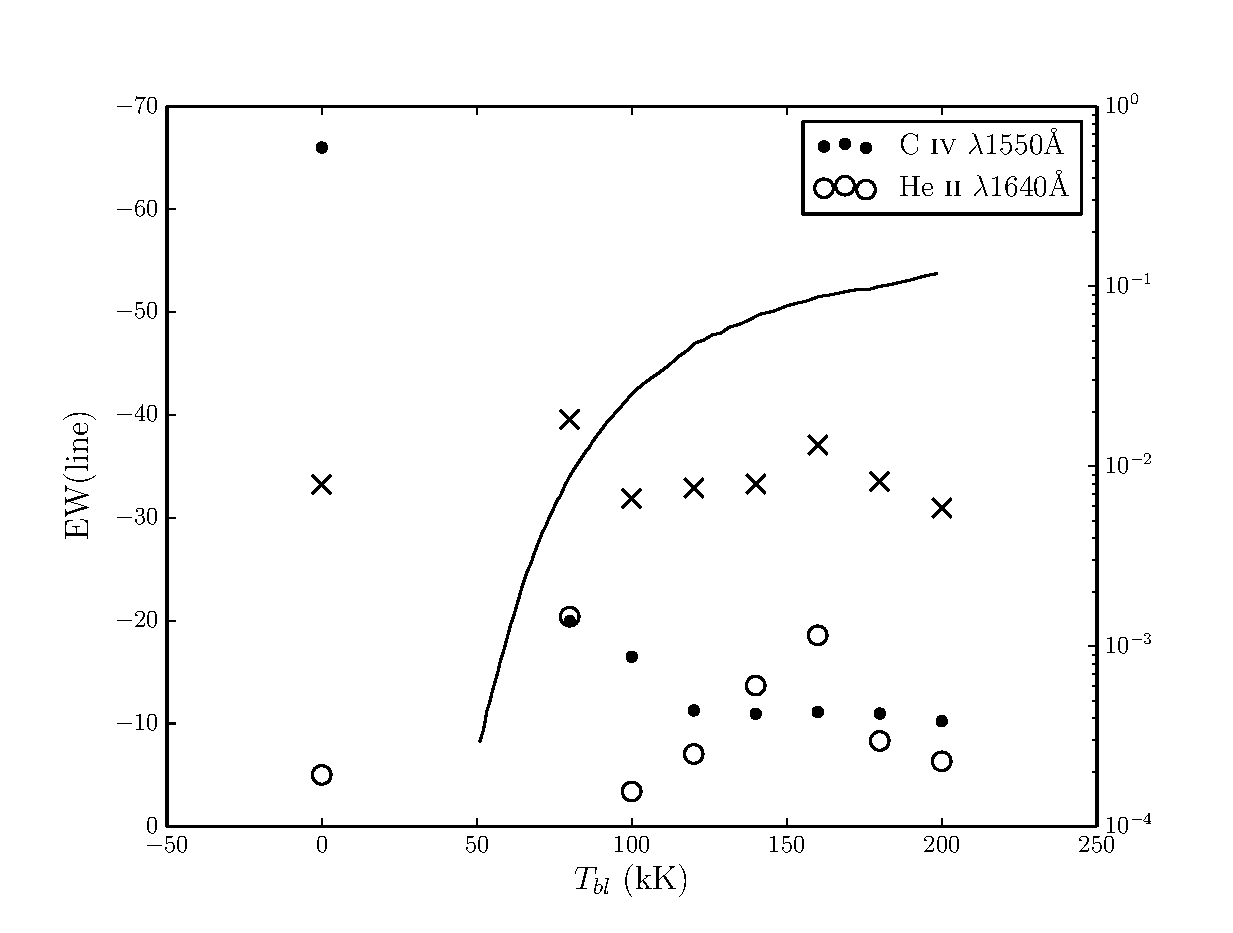
\includegraphics[width=0.5\textwidth]{figures/fig_EWt.eps}}

}
%%\includegraphics[width=0.5\textwidth]{figures/test.eps}
\caption{
Equivalent widths of the \civfull\ and \heiiuv\ lines
as a function of boundary layer temperature. The models used
are identical to the benchmark model in geometry and kinematics.
{\bf NOTE: The increase of He II line around 160kK is something we need to understand!}.
% The panels are ordered in the same way as figure~\ref{halpha}. In general, increasing densities
% lead to a Balmer jump in emission, although as in the case of H$\alpha$ there is a transition
% when the wind becomes a neutral absorbing column.
}
\label{bl_grid}
\end{figure}


% \noindent\rule{16cm}{0.4pt}

% {\bf
% \noindent Notes on Section 5:

% \begin{itemize}
% 	\item 

% \noindent Potential Additional Figures:

% \begin{itemize}
% 	\item 	
% }

% \noindent\rule{16cm}{0.4pt}

% \subsection{UV Resonance Lines}
% Compare spectra to LK02 and other models. Are the spectral features preserved, has anything significant changed.
% Lyman alpha?



% \subsection{Boundary Layer}
% \begin{itemize}
% \item discuss the effect of 80000K and 200000K Boundary layers
% \item Particularly referring to He II and CIV
% \item Our findings support idea that 200000K BL would over ionize the wind- 
% we favour 80,000K
% \item I'd like to do a hypothetical Zanstra calculation here- state what
% temperature our model would predict from the Zanstra method
% \end{itemize}

%\subsubsection{The Line Force}
%\begin{itemize}
%\item Can this wind be radiatively driven? 
%\item Why/why not?
%\item Figure showing line force throughout the wind as a fraction of some critical value?
%\end{itemize}


%%%%%%%%%%%%%%%%%%%%%%%%%%%%%%%%%%%%%%
%
%          Comparison with real spectra
%
%%%%%%%%%%%%%%%%%%%%%%%%%%%%%%%%%%%%%%%

\section{An Improved Optical Model }

\begin{table}
\centering
\begin{tabular}{p{3cm}p{4cm}}
Model B \\
\hline Free Parameters 	&	 Value \\ 
\hline \hline 
$M_{WD}$ 	 &	 $0.8 M_{\odot}$ \\ 
$\dot{M}_{acc}$ 	 &	 $10^{-9}~M_{\odot}yr^{-1}$\\ 
$\dot{M}_{wind}$  &	$10^{-8}~M_{\odot}yr^{-1}$\\ 
$r_{min}$ 	&	 $4 R_{WD}$\\ 
$r_{max}$ 	&	 $12 R_{WD}$ \\ 
$\theta_{min}$ 	&	 $20.0^{\circ}$ \\ 
$\theta_{max}$ 	&	 $65.0^{\circ}$ \\ 
$\gamma$ 	&	 $1$ \\ 
$v_{\infty}$ 	&	 $3v_{esc}$ \\ 
$R_v$ 	        &	 $142.9 R_{WD}$ \\ 
$\alpha$ 	&	 $4$ \\
\end{tabular}
\centering
\caption{Wind geometry parameters used in the next-generation CV model.}
\label{modelb}
\end{table}

With modest changes to the kinematics of the benchmark CV model,
it is possible to produce a model
that comes closer to reproducing the observed optical spectrum
of a Nova-like variables. The parameters for this model (imaginatively dubbed Model B)
are show in table~\ref{modelb}, and the synthetic spectrum
is shown in figure~\ref{uvoptb}. An in and out of eclipse comparison 
between the synthetic spectrum
at an angle of $80^\circ$ and the high-inclination nova-like RW Tri 
is also shown in figure~\ref{rwtricomp}. The inclination
for RW Tri has been disputed, with claimed values of $75^\circ$ \citep{groot2004},
$70.5^\circ$ \citep{smak1995}, $80^\circ$ \citep{longmore1981} and 
$82^\circ$\citep{frankking1981}. A lower inclination
would mean that our model would simply require lower densities 
and smaller emission regions to produce the required continuum level
and single peaked emission, so our conclusions from this comparison are
not particular sensitive to the value chosen.
We also emphasize that this is no sense a fit to the data. The model
is purely designed to reproduce the general behaviour of nova-likes
and give an indication of the likely densities and kinematics 
required in the wind.
%quotes a figure of , whereas  halevinhenden2008

The similarity with the observed spectrum is striking. 
Model B produces strong emission in all the Balmer lines, 
with line to continuum ratios
comparable to those in RW Tri. 
The line to continuum ratio increases during eclipse,
as one expects if the emission is produced in a disk wind, 
thereby mimicking the behaviour of SW Sex stars.
The single-peaked \ha\ line is produced by our models with a 
very similar width to the observed spectrum, although it is perhaps slightly more
`flat-topped' in the synthesized data.

One of the limitations of the model is that, apart 
from in H$\alpha$, the lines are in general double-peaked. 
The lack of high-resolution data in this regard makes detailed analysis difficult,
but it would appear that understanding how single-peaked 
line emission forms and the kinematics and densities required to
modify the line profile is still an open question. 
The major fallback of the next-generation model, however, lies
in the ultraviolet. To get the required emission in the optical lines
and recombination continuum the densities required are very high 
($n_e\sim10^{13}-10^{14}$ in the main emission region).
This causes a significant collisionally excited contribution
to the UV lines, meaning that the red wing of the 
resonance species such as C\textsc{iv} no longer matches the
observed profiles. 




\begin{figure} %fullpage
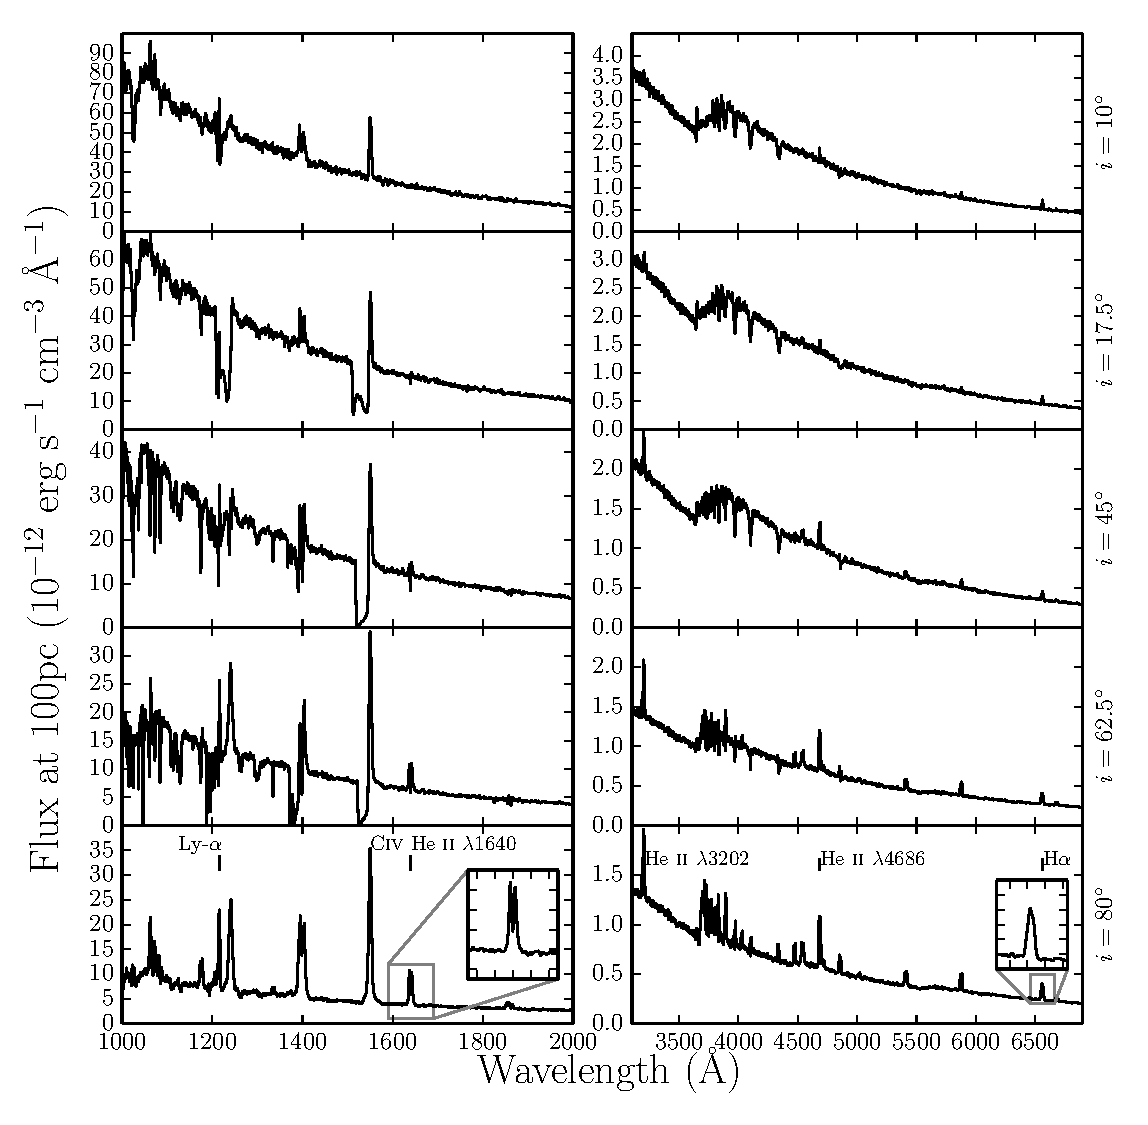
\includegraphics[width=\textwidth]{figures/fig14_uv_opt.eps}
\caption{
UV (left) and Optical synthetic spectra for model B computed at
sightlines of 10, 27.5, 45, 62.5 and 80 degrees.	
The inset plots show zoomed-in line profiles for 
\heiiuv \ and \ha. The \ha line 
is single peaked, but higher order lines in the Balmer series
are double-peaked, albeit with narrower profiles.
Strong \heiiopt emission can be seen, as well a trend
of a deeper Balemr jump with decreasing inclination.
}
\label{uvoptb}
\end{figure} %fullpage


\begin{figure} %fullpage
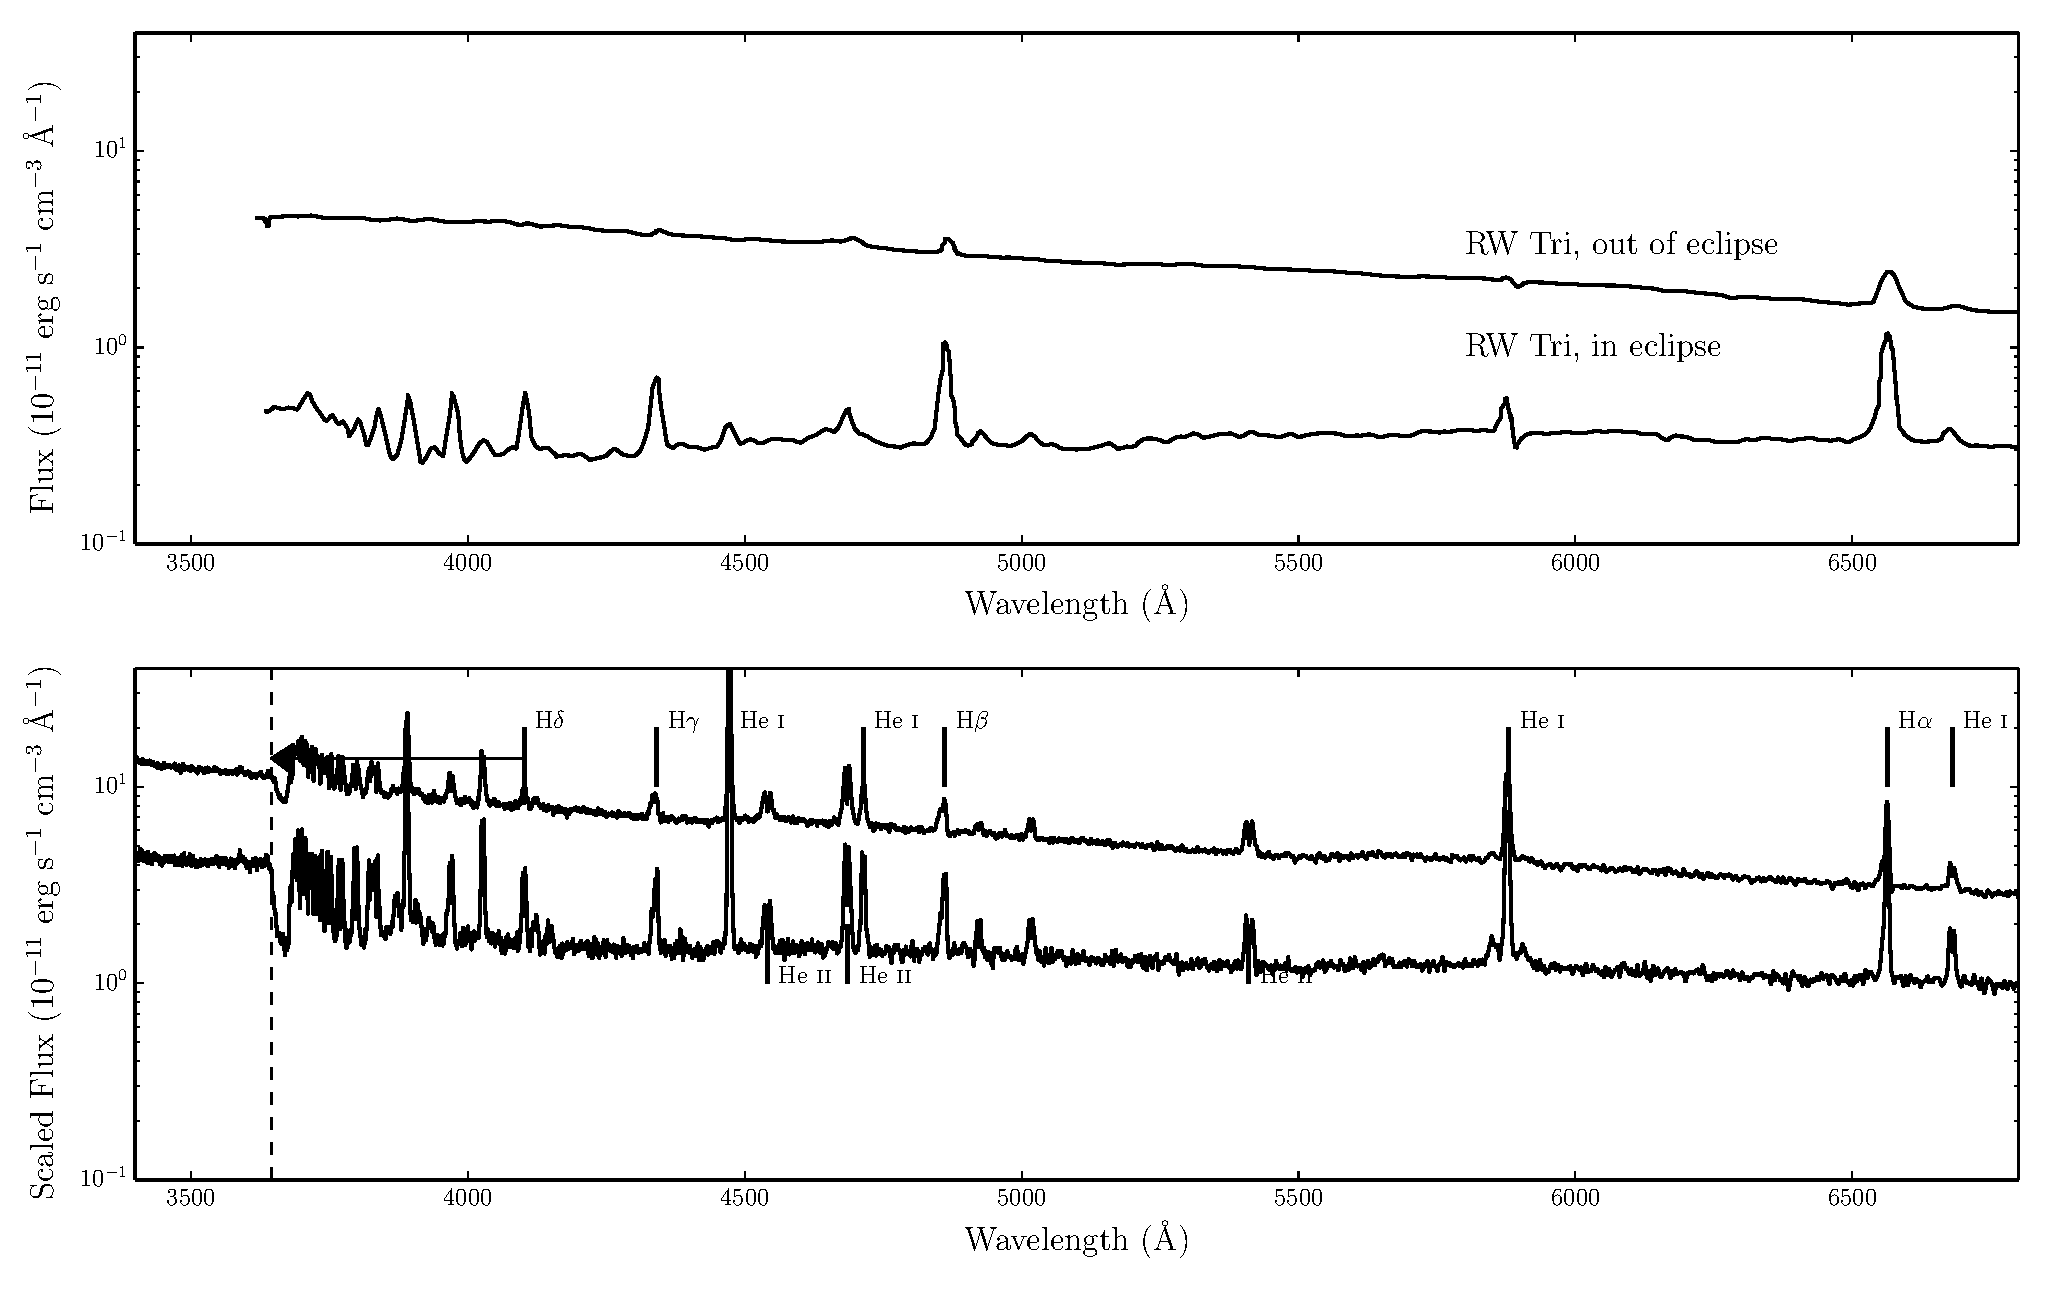
\includegraphics[width=0.8\textwidth]{figures/fig13_eclipse.eps}
\caption{{\sl Top Panel:} In and out of eclipse spectra of the high
inclination Nova-like RW Tri. {\sl Bottom Panel:} In and out of eclipse synthetic
spectra from Model B.}
\label{rwtricomp}
\end{figure} %fullpage


% \noindent\rule{16cm}{0.4pt}

% {\bf
% \noindent Notes on Section 6:

% \begin{itemize}
% 	\item 

% \noindent Potential Additional Figures:

% \begin{itemize}
% 	\item 	
% }

% \noindent\rule{16cm}{0.4pt}

%%%%%%%%%%%%%%%%%%%%%%%%%%%%%%%%%%%%%%
%
%          Conclusions and Future Work
%
%%%%%%%%%%%%%%%%%%%%%%%%%%%%%%%%%%%%%%%


\section{Conclusions}

By taking an already successful model
for the UV wavelength regime of CVs and treating 
it with an improved line transfer scheme, we have shown
that the wind does produce some recombination lines
and continuum emission blueward of the Balmer edge.
We have confirmed a number of the expected trends
by exploring a limited number of parameters governing the
kinematics and geometry of the wind. These include:

\renewcommand{\labelitemi}{$\bullet$}
\begin{itemize}
	\item The `filling-in' of the Balmer jump \citep{KLWB98} by recombination 
	continuum emission from a disk wind
	\item Single peaked line emission in \ha\ produced by 
	the introduction of a poloidal velocity gradient \citep{MC96}
	\item A Balmer decrement consistent with optically thick emission \citep{elitzur1983}.
\end{itemize}
\smallskip

\noindent We also make a number of predictions:

\begin{itemize}
	\item The depth of the Balmer absorption edge decreases with increasing inclination,
or alternatively that the Balmer recombination emission
is enhanced at higher inclinations, {\sl relative to the disk continuum}.
	\item The He~\textsc{ii}~$\lambda3202{\rm \AA}$ line should be
prominent in cases where He~\textsc{ii}~$\lambda1640{\rm \AA}$ \& 
\heiiopt\ are seen. 
	\item A Balmer jump in emission during eclipse.
\end{itemize}

\smallskip
We have presented a next-generation model
which produces all the prominent lines in and out of eclipse, and
shown that the model exhibits verisimilitude with the optical spectrum of RW Tri.
However, this model does not produce a complete unified CV model. 
The emission lines in the UV are somewhat unrealistic in strength,
because the high densities needed to increase line opacity also produce
a significant collisionally excited contribution..
This is a shortcoming which must be understood if it is true that
disk winds modify line profiles to become single peaked.
% as the 
%densities required produce a large amount of collisionally excited emission
%in UV resonance lines.

Our work demonstrates that, if nothing else,
{\sl disk winds matter}. At a minimum,
they can act as a spectral filter
for the disk spectrum
%and the properties of the plasma
%is an important tracer for the disk and boundary layer SEDs. 
At a maximum, they may be responsible
for the majority of spectral features of high-state CVs,
and could dominate the appearance of both UV and optical
spectra of these systems.

%% Balmer jump

% {\bf
% \noindent Notes on Section 7:

% \begin{itemize}
% 	\item 

% \noindent Potential Additional Figures:

% \begin{itemize}
% 	\item 	
% }


% \subsection{Future Work}

% To further investigate the true effect of the wind
% we hope that high quality, broadband spectra of 
% Nova-like variables at a range of inclinations 
% will be taken to examine 

% In addition to this project, we have started to apply the macro atom scheme to QSOs in order to build on the work of Higginbottom et al. (2013). In particular, we hope that the macro-atom scheme will enable the
% model to produce significant Lyman-$\alpha$ emission, as is observed in QSOs.


\subsection*{Acknowledgements}
The work of JHM, NH and CK is supported by the Science and Technology Facilities Council (STFC), 
via studentships and a consolidated grant, respectively. We would like to thank Juan Hernandez Santisteban and Ivan Hubeny 
for useful discussions. We acknowledge the use of the IRIDIS High Performance Computing Facility, 
and associated support services at the University of Southampton, in the completion of this work.


\newpage
\newpage
\bibliography{mybib.bib}

\end{document}
